\chapter{物理信息门控循环单元流变学本构方程建模研究}
% 3.2表================================================
% % 本节仅展示使用常见的三线表
% \begin{table}
%   \TableBicaption{\label{TDF_para}涵道模型参数}{Parameters of Ducted Fan Model}  % 中英文标题
%   \centering
%   \small
%   \begin{tabularx}{\textwidth}{XXXX}  % 使用 tabularx 环境,均匀分布列宽
%     \Xhline{1.5pt}
%     参数符号       & 数值                 & 参数符号  & 数值                 \tabularnewline
%     \Xhline{0.5pt}  % 表头下方线
%     $I_x$      & $054593$           & $I_y$ & $0.017045         $ \tabularnewline
%     $l_1$      & $0.0808\,\text{m}$ & $l_2$ & $0.175\,\text{m}  $ \tabularnewline
%     $l_4$      & $0.2415\,\text{m}$ & $l_5$ & $0.1085\,\text{m} $ \tabularnewline
%     $l_\sigma$ & $xdf$              & $df$  & 扫描电镜 \tabularnewline
%     \Xhline{1.5pt}
%   \end{tabularx}
% \end{table}
\section{引言}
近年来,深度学习在流变学本构建模研究中得到广泛应用。例如Lennon、Mahmoudabadbozchelou等人的研究工作,虽然具体方法各有不同,但在模型选择上基本都采用了多层感知机模型(Multi-Layer Perceptron,MLP)\cite{lennonScientificMachineLearning2023a,mahmoudabadbozchelouDatadrivenPhysicsinformedConstitutive2021}。MLP是一种经典的前馈人工神经网络,由输入层、多个隐藏层及输出层的全连接层堆叠而成,通过非线性激活函数实现复杂函数逼近。当MLP的隐藏层数达到一定值时,它被视为深度神经网络(Deep Neural Network,DNN)。传统的前馈性质DNN模型虽具备一定的非线性行为捕捉能力,但在处理具有时间依赖性的数据时,其性能往往受到限制。Lennon和Mahmoudabadbozchelou的工作使用DNN模型,难以有效捕捉黏弹性材料中的长程应变历史依赖性。本章研究在前人基础上,采用物理信息门控循环单元(Physical Information Gated Recurrent Unit,PI-GRU)进行本构建模,旨在解决DNN模型在处理时间序列数据时性能受限的问题。PI-GRU模型创新性地结合了物理约束和GRU的循环神经网络架构,通过在损失函数中引入物理方程残差作为惩罚项,同时利用GRU的循环结构处理时序数据。该模型包含输入层感知机、GRU循环层和输出层感知机三部分组成,输入为应变张量分量、应变速率张量分量和时间等参数,输出为预测的应力张量。

本章研究首先通过数值模拟方法构建了多种经典本构方程的应力应变数据,包括Herschel-Bulkley模型、Maxwell模型、Doi-Edwards模型。这些模型在流变学领域具有重要的理论和应用价值,能够描述不同类型的流变行为。随后,本章详细设计了GRU模型的结构、参数初始化及训练优化策略,并使用数值模拟生成的应力应变数据进行训练和参数优化,使模型能够准确拟合训练数据。为了验证GRU模型在探索未知流变学本构方程方面的能力,本章将训练好的GRU模型应用于未经训练的测试集数据,并通过与传统DNN等基准模型的对比,验证了GRU模型在处理时间序列数据方面的优势。在此基础上,本章进一步研究了更复杂的非线性本构关系,通过数值模拟方法生成Giesekus模型数据,并引入物理信息约束,构建PI-GRU模型进行建模。通过与其他基准模型的对比,验证了PI-GRU模型在复杂非线性本构关系建模中的有效性。最后,本章使用一类黏弹性聚合物的真实流变学实验数据进行PI-GRU训练和测试,进一步验证了该模型在真实工况下的适用性和优越性。
\section{深度学习模型设计}
本章针对Herschel-Bulkley模型、Maxwell模型、Doi-Edwards模型使用GRU模型进行建模,其基本架构在第二章已经详细介绍。
本章针对Giesekus模型和真实实验数据使用的算法模型PI-GRU模型,PI-GRU与基本的GRU神经网络模型架构类似,但不同的是,PI-GRU循环神经网络模型在GRU的基础上,加入了物理约束损失,用于约束模型的预测结果符合基本的本构物理规律,增强模型的泛化能力。
\begin{figure}
  \centering
  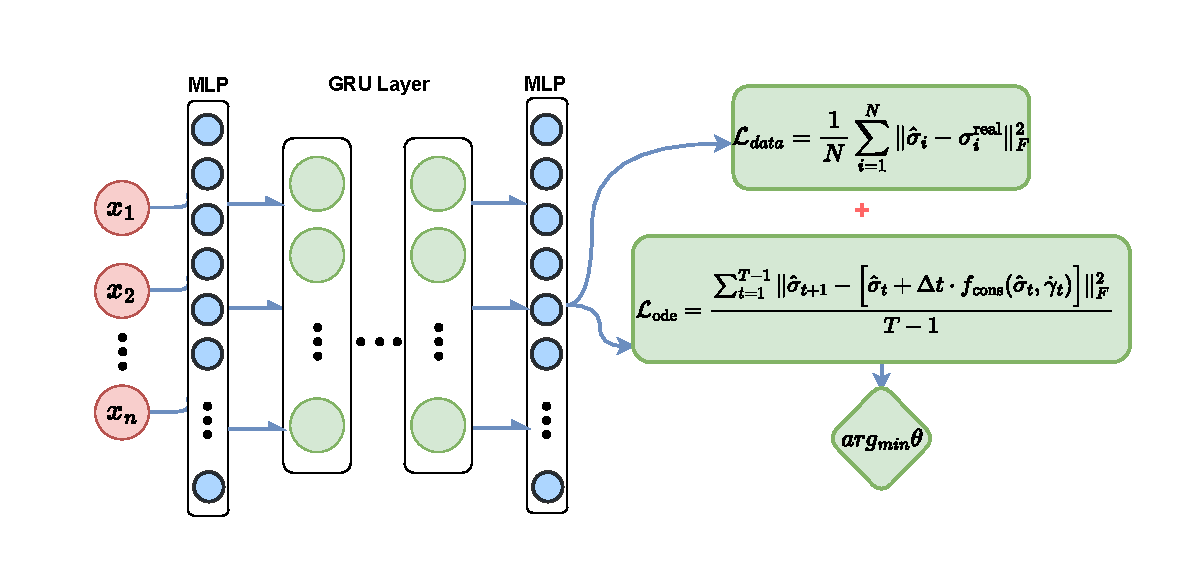
\includegraphics[width=0.9\textwidth]{Fig/PI-GRU.pdf}
  \FigureBicaption{\label{PI-GRU}本工作使用的PI-GRU架构示意图}{Schematic of the PI-GRU model used in this work}
\end{figure}
其架构图如图\ref{PI-GRU}所示,模型的输入为应变张量分量、应变速率张量分量、时间等,首先经过输入层的感知机进行特征提取,然后经过GRU层进行时序信息处理,最后经过输出层的感知机输出预测的应力张量。
PI-GRU的损失函数主体由数据损失和物理约束损失共同组成,具体公式如\ref{eq:pigru-loss-function}所示。
\begin{equation}
  \mathcal{L}_{\text{total}} =
  \lambda_{\text{data}} \mathcal{L}_{\text{data}} +
  \lambda_{\text{ode}} \mathcal{L}_{\text{ode}} +
  \lambda_{\text{dae}} \mathcal{L}_{\text{dae}}+
  \mathcal{L}_{L_{2}} \label{eq:pigru-loss-function}
\end{equation}
其中数据损失$\mathcal{L}_{\text{data}}$是预测值与真实值的均方误差(公式\ref{eq:data-loss}),目的是确保模型的预测结果与数值模拟数据尽可能接近,这是监督学习的基础,直接拟合数据,也是最重要和最基本的损失项。
\begin{equation}
  \mathcal{L}_{\text{data}} = \frac{1}{N} \sum_{i=1}^N
  \|\hat{\bm{\sigma}}_i - \bm{\sigma}_i^{\text{real}}\|_F^2
  \quad \label{eq:data-loss}
\end{equation}

\begin{equation}
  \mathcal{L}_{\text{ode}} = \frac{1}{T-1} \sum_{t=1}^{T-1}
  \|\hat{\bm{\sigma}}_{t+1} - \Bigl[
    \hat{\bm{\sigma}}_t + \Delta t \cdot
    f_{\text{constitutive}}(\hat{\bm{\sigma}}_t, \dot{\gamma}_t)
    \Bigr] \|_F^2
  \quad \label{eq:ode-loss}
\end{equation}
物理损失分为ODE损失$\mathcal{L}_{\text{ode}}$和DAE损失$\mathcal{L}_{\text{dae}}$。$\mathcal{L}_{\text{ode}}$确保模型的预测遵循本构方程描述的物理规律,如公式\ref{eq:ode-loss}所示。该公式计算的是时间序列中相邻时间步之间的平均损失,其中$\hat{\bm{\sigma}}_{t+1}$是模型在$t+1$时刻的预测应力,而方括号内的表达式$\hat{\bm{\sigma}}_t + \Delta t \cdot f_{\text{constitutive}}(\hat{\bm{\sigma}}_t, \dot{\gamma}_t)$是根据本构方程从$t$时刻推导出的$t+1$时刻的理论应力值。这种损失函数通过比较模型预测值与基于物理定律推导值之间的差异,确保模型学习结果符合我们想要的本构关系。这里的本构方程在Giesekus模型模拟数值训练时为上对流Maxwell模型(UCM),在真实实验数据时为最小二乘法拟合的各类本构方程。

$\mathcal{L}_{\text{dae}}$损失则是为了保证预测的应力张量满足基本的对称性要求。物理损失相当于一个独特的惩罚机制,迫使模型的预测结果约束在基本的框架内,一定程度上防止模型在纯数据驱动下出现过拟合现象。
\begin{equation}
  \mathcal{L}_{\text{dae}} = \frac{1}{T} \sum_{t=1}^T \Biggl(
  \underbrace{\|\hat{\bm{\sigma}}_t - \hat{\bm{\sigma}}_t^\top\|_F^2}_{\text{symmetry constraint}}
  \Biggr)
  \quad \label{eq:dae-loss}
\end{equation}
\begin{equation}
  \mathcal{L}_{L_{2}} = \lambda \sum_{i} w_i^2
  \quad \label{eq:l2-loss}
\end{equation}
最后在损失函数中加入正则化项$\mathcal{L}_{L_{2}}$,具体公式如公式\ref{eq:l2-loss}。$\mathcal{L}_{L_{2}}$通过类似于归纳推理的机制,使得模型倾向于学习更通用的模式,参数更小更简单,对未知数据的预测更可靠。

\section{实验设计}
\subsection{数据获取}
\subsubsection{Herschel-Bulkley模型模拟数据}
Herschel-Bulkley模型的本构方程如公式\eqref{eq:herschel}所示,其中剪切应力$\sigma$与剪切率$\dot{\gamma}$之间存在函数关系。该模型包含流变参数$K$、流动指数$n$及屈服应力$\sigma_0$。在模拟过程中,本章设置$\sigma_0$为1.0 Pa,$K$为1,而$n$则取值为0.2、0.6、1.0、1.4及1.8。剪切率$\dot{\gamma}$范围设定为[0,100],并以0.01的时间步长进行离散采样。

数据生成后,本章首先采用Matplotlib库绘制出剪切应力$\sigma$与剪切率$\dot{\gamma}$的关系曲线,观察模拟效果,并进行生成效果评估。随后本章采用NumPy库进行数据处理,使用Pandas库将数据存储为Excel文件,便于后续的模型训练。
\subsubsection{Maxwell模型模拟数据}
Maxwell模型的微分本构方程如公式\eqref{eq:maxwell_model_dt}所示。该模型包含松弛时间$\tau=\eta/G$,其中$\eta$表示黏性系数,$G$为剪切模量。本章设置$\eta$为0.1 Pa·s,$G$为1.0 Pa。采用后向欧拉法来离散化微分方程,具体推导如下:

首先将微分离散化,设$d\sigma=\sigma_i - \sigma_{i-1}$,$dt=\Delta t$,$d\gamma=\gamma_i - \gamma_{i-1}$,则原方程可以化简为公式\eqref{eq:maxwell_euler_back_1},
\begin{equation}
  \frac{\sigma_i - \sigma_{i-1}}{\Delta t} + \frac{\sigma_i}{\tau} = G \frac{\gamma_i - \gamma_{i-1}}{\Delta t} \label{eq:maxwell_euler_back_1}
\end{equation}
移项并化简可得公式\eqref{eq:maxwell_euler_back_2}。
\begin{equation}
  \sigma_i = \frac{\sigma_{i-1} + G (\gamma_i - \gamma_{i-1})}{1 + \frac{\Delta t}{\tau}} \label{eq:maxwell_euler_back_2}
\end{equation}
根据公式\eqref{eq:maxwell_euler_back_2},本章首先使用NumPy库生成6个不同应变变化协议的应变数据,时间步为0.01 s,每个协议模拟2000个数据点,并存为NumPy数组,随后通过迭代法计算单个应变数据对应的应力数据,并存为NumPy数组。之后,本章使用Matplotlib库绘制出剪切应力与剪切应变的关系曲线,观察模拟效果,并进行生成效果评估。最后本章使用Pandas库将数据存储为Excel文件,便于后续的模型训练。
\subsubsection{Doi-Edwards模型模拟数据}
Doi-Edwards模型的本构方程如公式\eqref{eq:doi_edwards}所示。该方程为积分形式的本构方程,本章首先对该方程进行处理,将取向张量函数$\mathbf{Q}(t^{\prime},t)$写为球坐标形式,即公式\eqref{eq:doi_edwards_moni_q}。
\begin{align}
   & \mathbf{Q}(t^{\prime},t) = \frac{1}{4\pi} \int_{0}^{2\pi} \int_{0}^{\pi} 5 \left( \frac{\mathbf{u}^{\prime} \cdot \mathbf{F}^{-1} \mathbf{u}^{\prime} \cdot \mathbf{F}^{-1}}{|\mathbf{u}^{\prime} \cdot \mathbf{F}^{-1}|^{2}} \right) \sin\theta \, d\theta \, d\phi   \label{eq:doi_edwards_moni_q} \\
   & G(t, t') = \frac{G_0}{\lambda_i} \exp\left( \frac{t' - t}{\lambda_i} \right)   \label{eq:doi_edwards_moni_g}                                                                                                                                                                                         \\
   & \boldsymbol{\sigma}(t) = \int_{t_0}^t G(t, t') \cdot \mathbf{Q}(\gamma(t')) \, dt' \label{eq:doi_edwards_moni_sigma}
\end{align}

本章模拟的为简单剪切流动,只在xy方向存在应变,因此可以将逆变形梯度张量$\mathbf{F}^{-1}$写为公式\eqref{eq:doi_edwards_f_inverse}的矩阵形式,$\mathbf{u}^{\prime}$为球坐标系下的单位向量。
\begin{equation}
  \mathbf{F}^{-1} = \begin{bmatrix}
    1      & 0 & 0 \\
    \gamma & 1 & 0 \\
    0      & 0 & 1
  \end{bmatrix} \label{eq:doi_edwards_f_inverse}
\end{equation}
公式\eqref{eq:doi_edwards_moni_g}为松弛模量函数,本章使用NumPy库生成7个不同的应变协议的NumPy数组,单个协议时间区间为[0,4$\pi$],总数据点为2000个,生成形式为3$\times$3的张量矩阵,代入公式\eqref{eq:doi_edwards_moni_q}计算$\mathbf{Q}$值数组。设置$G_0$为1.0 Pa,$\lambda$为1.0 s,$i=1$,根据公式\eqref{eq:doi_edwards_moni_sigma}计算应变张量,使用的积分工具为Python的scipy.integrate库,生成形式为3$\times$3的张量矩阵,如公式\eqref{eq:sigma_bmatrix}所示。本章提取$
  \sigma_{12}$、$\sigma_{11}$、$\sigma_{22}$分量作为模拟实验数据,与对应的应变分量数据一起通过Pandas库存入Excel文件,便于后续的模型训练。
\begin{equation}
  \boldsymbol{\sigma} = \begin{bmatrix}
    \sigma_{11} & \sigma_{12} & \sigma_{13} \\
    \sigma_{21} & \sigma_{22} & \sigma_{23} \\
    \sigma_{31} & \sigma_{32} & \sigma_{33}
  \end{bmatrix} \label{eq:sigma_bmatrix}
\end{equation}
\subsection{Giesekus模型模拟数据}
Giesekus模型的本构方程如公式\eqref{eq:giesekus}所示,迁移因子$\alpha$用于引入剪切稀化的强度。Giesekus模型模拟的为简单剪切流动,只在xy方向存在应变,应变张量$\boldsymbol{\gamma}$仅在$\gamma_{12}$分量上存在值。
本章首先使用NumPy库生成不同速度场协议的简单剪切流动速度数据,再使用公式\eqref{eq:giesekus-gammadot}对应生成应变速率张量数据,单个协议的模拟数据点为2000,生成形式为3*3应变速率张量矩阵,之后根据$\gamma_{t}=\dot{\gamma}_{t-1}\Delta t+\gamma_{t-1}$迭代计算应变张量。
\begin{equation}
  \begin{aligned}
    \dot{\gamma}_{ii} & = 2 v_{ii}(t)           \\
    \dot{\gamma}_{ij} & = v_{ij}(t) + v_{ji}(t)
  \end{aligned} \label{eq:giesekus-gammadot}
\end{equation}
随后设置迁移因子$\alpha$为0.8,其余松弛时间参数($\lambda_1$、$\lambda_2$)为1.0,使用Python的scipy.integrate.solve\_ivp函数(内置方法为Runge-Kutta法)对Giesekus模型的微分方程组进行求解计算,生成3*3应力张量矩阵,如公式\eqref{eq:sigma_bmatrix}所示。本章提取$\sigma_{12}$、$\sigma_{11}$、$\sigma_{22}$分量作为模拟实验数据,与对应的应变速率张量数据、计算后的应变张量数据一起通过Pandas库存入Excel文件,便于后续的模型训练。
\subsubsection{真实实验数据}
首先通过原子转移自由基聚合(ATRP)和开环异位聚合(ROMP)设计了由聚甲基丙烯酸(亲水单元)和聚甲基丙烯酸叔丁酯(疏水单元)的两亲性刷状聚合物(ABPs),再将合成的两亲性分子刷溶解在DMF中,与甲氧基丙烯酸酯混合制成弹性体前驱体溶液,该前驱体溶液含有规定的总单体浓度6 mol/L (= [ABPs] + [MEA]),其中 MEA质量分数为90\%, ABPs质量分数为10\%,引发剂为总单体摩尔量的0.1\%的二苯甲酮,交联剂含量为总单体摩尔量的0.1\%的PEGDA。在氩气气氛中将混合溶液注入一个反应池,该反应池由平行玻璃板组成,由1.0毫米厚的硅胶垫片隔开。聚合反应在紫外光照射下进行8 h。将制备好的弹性体从反应池中取出,并在大量去离子水中浸泡至少24小时,去除未反应的单体,然后在真空烘箱中40℃干燥3天,得到均匀的两亲性刷掺杂的弹性体(ABE弹性体)。

通过安东帕型流变仪在25℃下测量具有0.8mm厚度的材料的振荡剪切试验。将样品置于8mm直径的平行板下,在1\%到300\%的应变范围内以10rad/s的固定频率对样品进行应变扫描。当正弦交变应变作用于材料时,材料发生相应的正弦交变应力,通过绘制振幅-模量曲线,可以得到材料的非线性区临界应变。
\subsection{模型训练}
\subsubsection{数据集划分}
首先本章对模拟生成的数据进行数据集划分,将数据集分为训练集(Train)、验证集(Valid)和测试集(Test)。其中每种本构模型数据集和真实数据数据集分别选取一组待预测数据作为测试集,其余数据按照9:1比例划分为训练集和验证集。


\subsubsection{训练细节}
本研究使用PyTorch框架进行模型训练,使用Adam优化器进行优化。超参数的设置采用随机搜索算法,该算法通过在预定义的超参数空间中进行随机采样来寻找最优组合。具体而言,对于学习率$\eta$,在对数空间[10$^{-5}$, 10$^{-2}$]内随机采样;batch size在{16, 32, 64, 128}中随机选择;隐藏层神经元数量在{10, 20, 30, 40}范围内随机采样。随机搜索的优化目标函数可表示为:

\begin{equation}
  \theta^* = \arg \min_{\theta \in \Theta} \mathcal{L}_{\text{val}}(f_\theta(X_{\text{val}}), y_{\text{val}})
\end{equation}

其中$\Theta$表示超参数空间,$\mathcal{L}_{\text{val}}$为验证集上的损失函数。

为了进一步提高训练效率,本文还采用了学习率自适应调整策略。具体使用带有预热(warmup)的余弦退火调度\cite{loshchilov2016sgdr},学习率$\eta$随训练轮次$t$的变化可表示为:

\begin{equation}
  \eta(t) = \begin{cases}
    \eta_{\text{max}} \cdot \frac{t}{T_{\text{warmup}}}                                                                                             & \text{if } t \leq T_{\text{warmup}} \\
    \eta_{\text{min}} + \frac{1}{2}(\eta_{\text{max}}-\eta_{\text{min}})(1+\cos(\frac{t-T_{\text{warmup}}}{T_{\text{total}}-T_{\text{warmup}}}\pi)) & \text{if } t > T_{\text{warmup}}
  \end{cases}
\end{equation}

其中$T_{\text{warmup}}$为预热期轮次数,$T_{\text{total}}$为总训练轮次,$\eta_{\text{max}}$和$\eta_{\text{min}}$分别为最大和最小学习率。这种策略既能避免训练初期不稳定,又可以在后期实现更精细的参数调整。
\subsection{模型测试}
模型验证首先通过可视化方法直观比较预测结果与真实值。主要采用预测值-真实值曲线对比和残差分析图两种可视化方式。预测值-真实值曲线对比将模型预测的应力-应变曲线与真实数据在同一坐标系中绘制,直观展示模型预测的准确性。残差分析图则计算每个时间点的预测值与真实值之间的差异(残差),并绘制残差随时间或应变的变化图,能够揭示模型预测中的系统性偏差。理想情况下,残差应随机分布在零线附近,不呈现明显的趋势或模式。

本章的模型训练均为回归问题,因此采用的测试指标包括决定系数(Coefficient of Determination,R$^2$),如公式\eqref{eq:r2}所示,平均绝对误差(Mean Absolute Error,MAE),如公式\eqref{eq:mae}所示,以及平均百分比误差(Mean Absolute Percentage Error,MAPE),如公式\eqref{eq:mape}所示。
\begin{equation}
  \text{R}^2 = 1 - \frac{\sum_{i=1}^{n} (y_i - \hat{y}_i)^2}{\sum_{i=1}^{n} (y_i - \bar{y})^2} \label{eq:r2}
\end{equation}
\begin{equation}
  \text{MAE} = \frac{1}{n} \sum_{i=1}^{n} |y_i - \hat{y}_i| \label{eq:mae}
\end{equation}
\begin{equation}
  \text{MAPE} = \frac{100\%}{n} \sum_{i=1}^{n} \left| \frac{y_i - \hat{y}_i}{y_i} \right| \label{eq:mape}
\end{equation}
此外,加上训练时间作为训练成本指标,全面评估模型性能。


\section{结果与讨论}
\subsection{Herschel-Bulkley模型建模}
\subsubsection{数值模拟数据}
\begin{figure}[htbp]
  \centering
  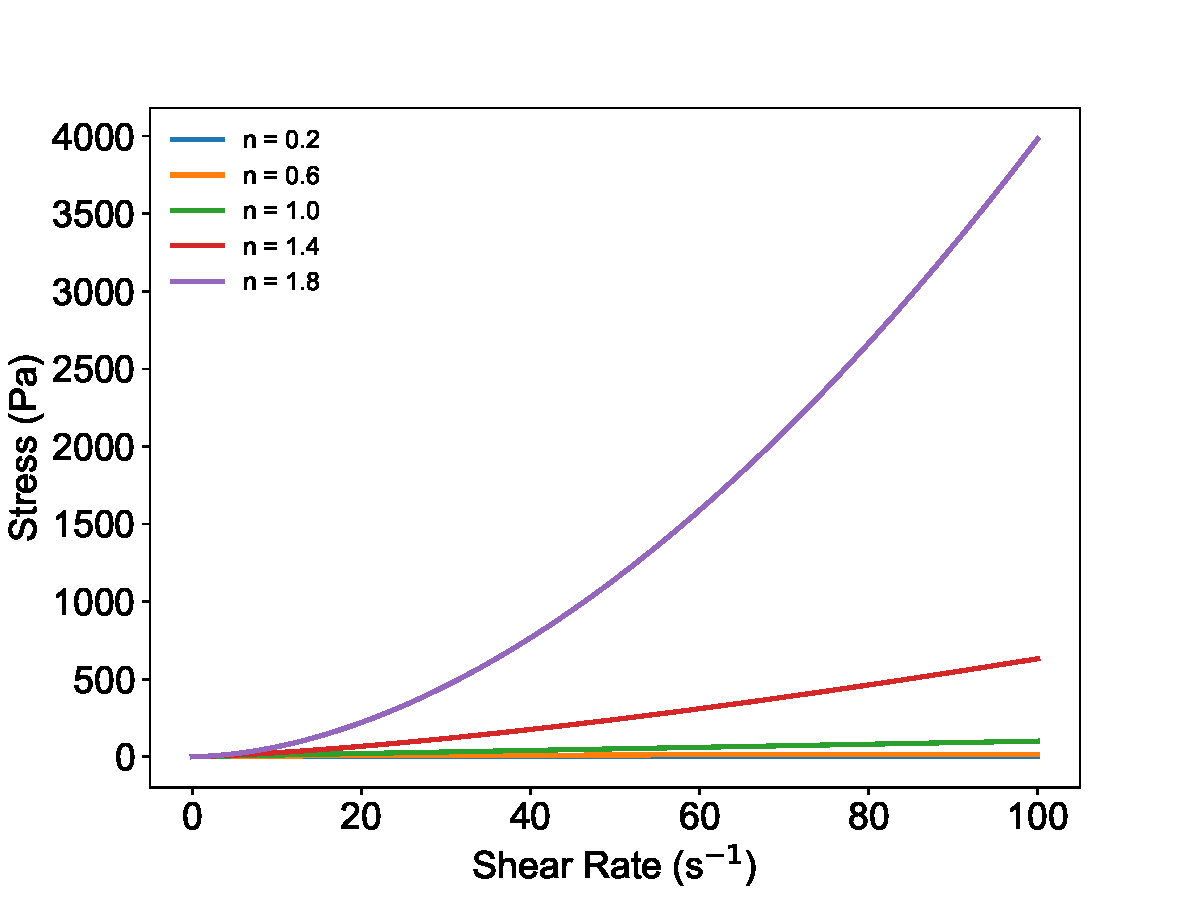
\includegraphics[width=0.8\textwidth]{Fig/herschel_moni.pdf}
  \FigureBicaption{\label{herschel_moni}Herschel-Bulkley模型模拟数据应力-应变率曲线图,n为流变指数}{Stress–strain rate curve of simulated data for the Herschel-Bulkley model, where n represents the flow index}
\end{figure}
本节使用Herschel-Bulkley模型模拟数据,模拟结果如图\ref{herschel_moni}所示。由图\ref{herschel_moni}可以看到,模拟数据中剪切应力Stress与剪切速率Shear Rate呈现幂函数关系,随着流变指数$n$的增加,曲线的斜率增大,表明流体的非牛顿特性增强。这一现象与Herschel-Bulkley模型的数学形式相符,说明模拟数据符合预期。
\subsubsection{GRU/DNN模型预测效果对比}

本节分别使用GRU和DNN两种算法对Herschel-Bulkley模型模拟数据进行深度学习建模,之后使用预测模型在测试集上进行验证,测试结果如图\ref{herschel_test}所示。图\ref{herschel_test}(a)为两种算法测试的真实值-预测值曲线,从曲线可以定性看出两种算法的预测值曲线与真实值曲线都非常接近。图\ref{herschel_test}(b)为两种算法测试结果的残差图,可以看出两种算法的残差点离散程度接近,均没有明显趋向性,均呈现无序分布,说明两种算法均可以比较好地捕捉到所有的输入特征。图\ref{herschel_test}(c-f)分别比较了两种算法预测结果的R$^2$,MAE,MAPE指标,从结果中可以看出,两种算法的预测效果都十分良好,R$^2$都接近1,GRU预测结果的R$^2$值略高于DNN,GRU预测结果的MAE和MAPE值都小于DNN,但数值差距不大。GRU算法的平均训练时间为378 s,高于DNN的155 s 一倍以上,这是由于GRU网络的参数量更大,且由于其循环神经网络的特点,只能顺序运算,限制了GPU的并行计算能力,导致训练时间较长。

综合看来GRU和DNN两种算法在Herschel-Bulkley模型模拟数据上的预测表现比较接近,从预测指标的绝对数值看,GRU略优于DNN。这个结果符合预期,因为Herschel-Bulkley模型本质上是模拟了剪切稀化增稠过程,不涉及黏弹性材料的时间依赖性,并且我们模拟的过程中,对于某个特定时间的应力状态也仅仅是当前应变状态的函数。从训练时间的分析看,GRU的训练成本远高于DNN。综合而言对于本构方程类似于Herschel-Bulkley模型的流体,GRU算法虽然在泛化效果上略有优势,但是综合性能上不具备显著优势。
\begin{figure}[H]
  \centering
  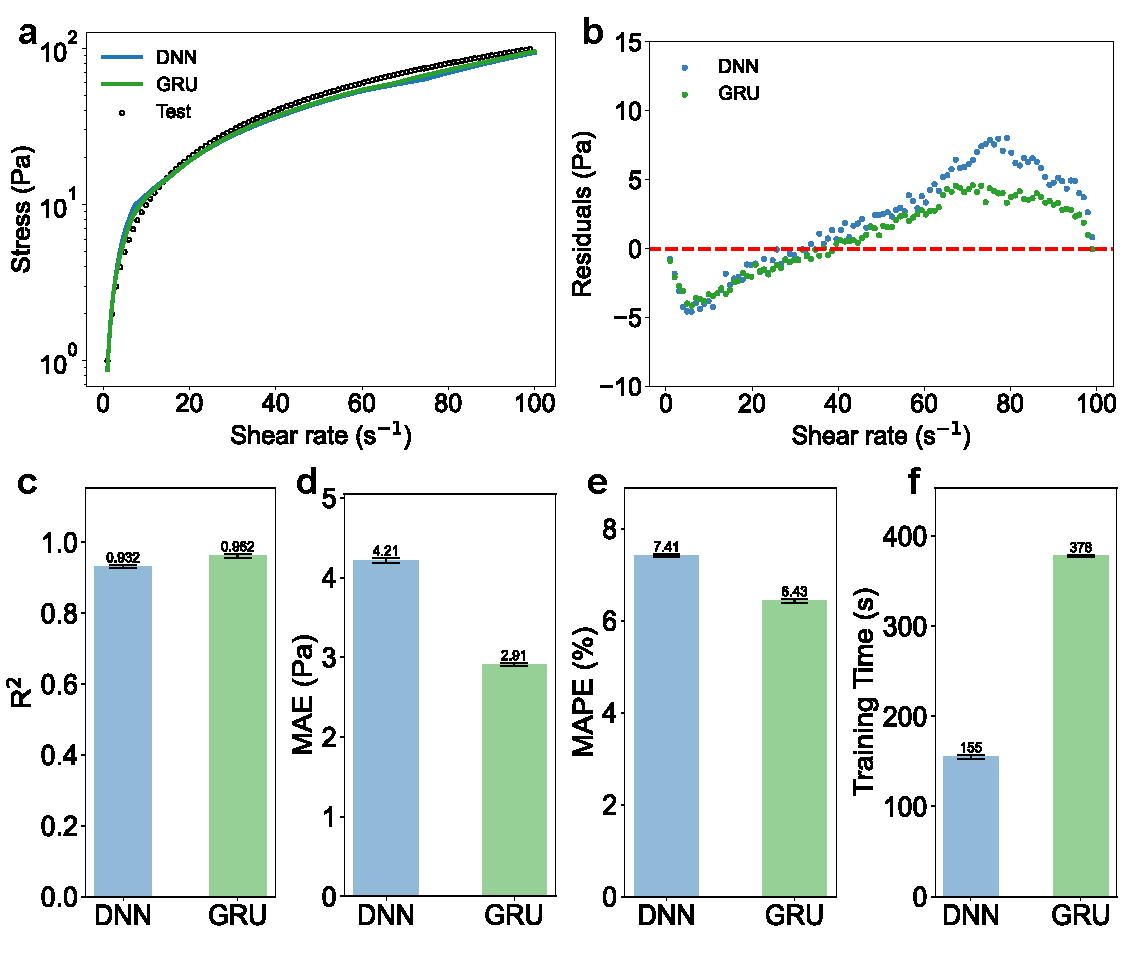
\includegraphics[width=0.8\textwidth]{Fig/Herschel_test.pdf}
  \FigureBicaption{\label{herschel_test}GRU算法和DNN算法在Herschel-Bulkley模型测试集上的预测效果对比示意图:(a)GRU和DNN在训练建模后的预测值-真实值曲线图;(b)GRU和DNN训练建模后的预测值残差图;(c)GRU和DNN测试集上的R$^2$指标图;(d)GRU和DNN在测试集上的MAE指标图;(e)GRU和DNN在测试集上的MAPE指标图;(f)GRU和DNN在测试集上的训练时间指标图}{Comparison schematic of the prediction performance of the GRU algorithm and the DNN algorithm on the Herschel-Bulkley model test set: (a) Predicted value–true value curves for GRU and DNN after training and modeling; (b) Residual plots of the predicted values for GRU and DNN after training and modeling; (c) R$^2$ metric plots on the test set for GRU and DNN; (d) MAE metric plots on the test set for GRU and DNN; (e) MAPE metric plots on the test set for GRU and DNN; (f) Training Time metric plots on the test set for GRU and DNN}
\end{figure}
\subsection{Maxwell模型建模}
\subsubsection{数值模拟数据}
\begin{figure}[htbp]
  \centering
  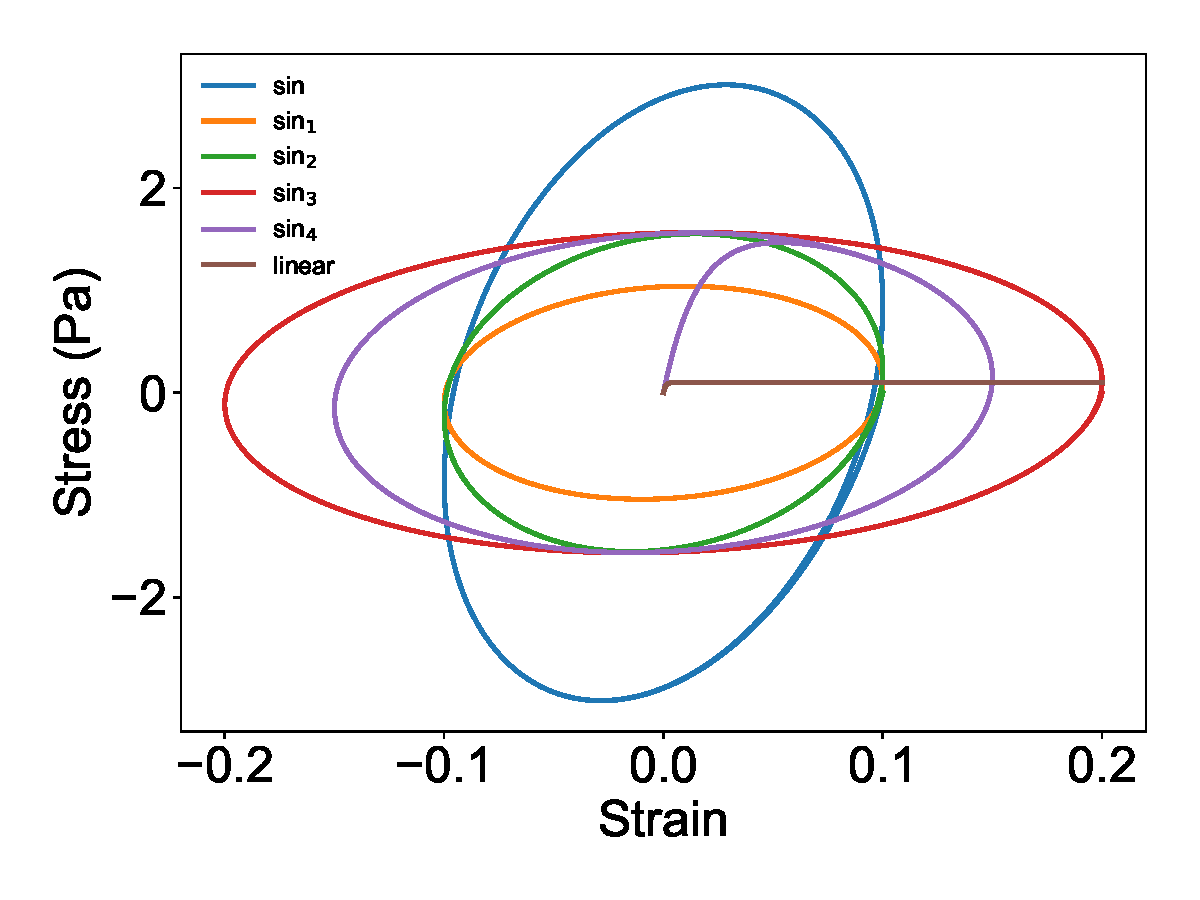
\includegraphics[width=0.8\textwidth]{Fig/maxwell_moni.pdf}
  \FigureBicaption{\label{maxwell_moni}不同应变变化协议的Maxwell模型模拟数据应力-应变曲线(Lissajous曲线)图}{Stress–strain curves (Lissajous curves) of simulated data for the Maxwell model under different strain variation protocols}
\end{figure}
本节通过后向欧拉法对简单 Maxwell 模型进行了数值模拟,生成了模拟数据,并绘制了应力-应变曲线(Lissajous 曲线),结果如图 \ref{maxwell_moni} 所示。图 \ref{maxwell_moni} 展示了不同应变协议下的模拟结果。对于正弦交变应变,Lissajous 曲线呈现出标准的闭合椭圆形状,这与 Maxwell 模型的理论预期一致,表明模型在周期性应变下的响应具有良好的稳定性和可预测性。对于线性应变,Lissajous 曲线在应变较小时表现出应力的快速增加,随后随着应变的继续增加,应力逐渐趋于一个稳定值,这一现象同样符合 Maxwell 模型的理论预期,反映了材料在持续应变下的应力松弛特性。综合看来,后向欧拉法模拟的数据符合预期,可以用于后续训练。


\subsubsection{交变预测交变效果验证}
\begin{figure}[htbp]
  \centering
  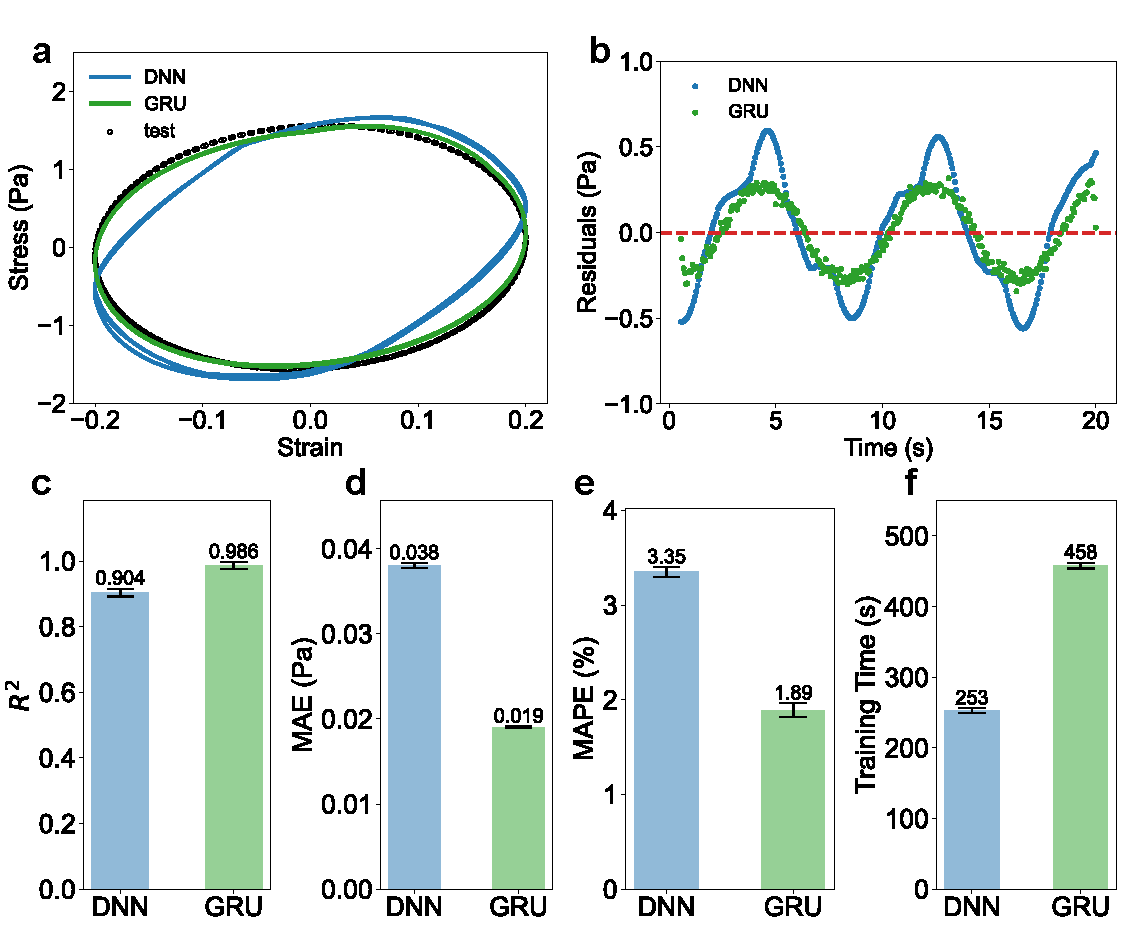
\includegraphics[width=0.8\textwidth]{Fig/Maxwell_sin_test.pdf}
  \FigureBicaption{\label{maxwell_sin}GRU算法和DNN算法在Maxwell模型交变协议测试集上的预测效果对比示意图:(a)GRU和DNN在测试集上的预测值与真实值的应力-应变曲线(Lissajous曲线);(b)GRU和DNN在测试集上的预测值与真实值的应力-时间曲线;(c)GRU和DNN在测试集上的预测值残差图}{Comparison of prediction performance between GRU and DNN algorithms on Maxwell model alternating protocol test set: (a) Stress-strain curves (Lissajous curves) of predicted vs. true values for GRU and DNN on test set; (b) Stress-time curves of predicted vs. true values for GRU and DNN on test set; (c) Residual plots of predicted values for GRU and DNN on test set}
\end{figure}
\begin{figure}[htbp]
  \centering
  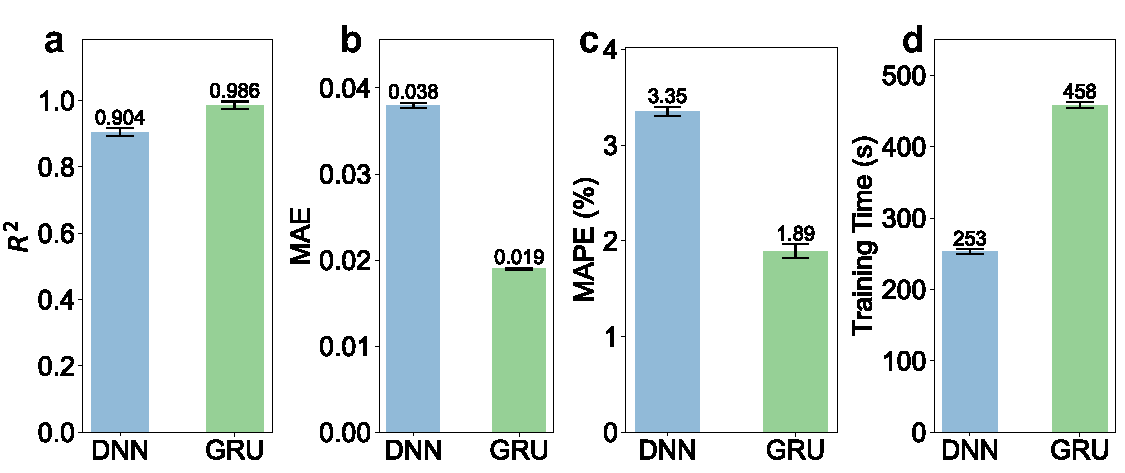
\includegraphics[width=0.8\textwidth]{Fig/Maxwell_sin_metric.pdf}
  \FigureBicaption{\label{maxwell_sin_metric}GRU算法和DNN算法在Maxwell模型交变测试集上的预测指标对比图:(a)GRU和DNN在测试集上的R$^2$指标图;(b)GRU和DNN在测试集上的MAE指标图;(c)GRU和DNN在测试集上的MAPE指标图;(d)GRU和DNN在测试集上的训练时间指标图}{Comparison schematic of the prediction performance of the GRU algorithm and the DNN algorithm on the Maxwell model alternating protocol test set: (a) R$^2$ metric plots on the test set for GRU and DNN; (b) MAE metric plots on the test set for GRU and DNN; (c) MAPE metric plots on the test set for GRU and DNN; (d) Training Time metric plots on the test set for GRU and DNN}
\end{figure}
为了验证GRU算法在时间序列本构方程数据中的预测效果,本节使用交变应变协议生成的数据作为训练集,交变应变协议生成的数据作为测试集。分别使用了GRU和DNN进行训练,并在测试集上进行验证,测试结果如图\ref{maxwell_sin}、图\ref{maxwell_sin_metric}所示。

图\ref{maxwell_sin}(a-b)为两种不同算法预测模型在测试集上的真实值-预测值曲线,
图a为Lissajous曲线,可以看到GRU算法的预测值的Lissajous曲线与真实值曲线十分接近,而DNN算法的预测值的Lissajous曲线与真实的曲线则有明显的周期性偏差,尤其在大应变时,预测值与真实值有较大的偏差。图b为时间-应力曲线,从中可以看到GRU算法的预测值曲线随时间变化较为稳定,贴近真实值曲线,而DNN算法的预测值的曲线明显偏离真实值曲线。

图\ref{maxwell_sin}(c)为两种算法预测模型的测试集残差图,从图中可以看到DNN算法的预测值与真实值残差呈现非常明显的周期性分布,极值偏离零刻度线,说明DNN模型无法泛化到测试集。而GRU的残差图虽然也存在一定周期性,但是总体分布效果明显优于DNN的对应残差,这说明GRU捕捉到了训练数据的较完整的特征,尤其是DNN未能捕捉的周期性特征。综合真实值-预测值曲线和残差图,可以定性分析出GRU的预测效果更为优秀。


接下来,本节计算两种算法的测试集预测指标,绘制指标对比图\ref{maxwell_sin_metric}。从图\ref{maxwell_sin_metric
}(a)显示,GRU的R$^2$值为0.986,接近1,说明GRU的预测效果十分优秀,而DNN的R$^2$值为0.904,略低于GRU,但是也高于0.9,属于非常出色的指标。仅从R$^2$指标来看,GRU预测效果优于DNN,但是优势不明显。从图\ref{maxwell_sin_metric}(b-c)看,GRU预测结果的MAE值为0.019,仅为DNN预测结果的MAE值的一半,GRU预测结果的MAPE值为1.89,仅为DNN预测结果的MAPE值3.35的一半。这定量说明GRU的预测结果误差远小于DNN的预测结果误差,GRU在此项任务上预测泛化效果更好。当然,由于GRU的模型特性,其训练时间如图\ref{maxwell_sin_metric}(d)所示,要高于DNN。

综合各项分析数据来看,当训练数据和测试数据为同类型应变变化过程(都为交变应变)时,GRU算法可以更好的学习到Maxwell模型数据的内在特征,包括周期性响应,黏弹性,时间依赖性响应。从定性与定量分析结果看,GRU算法的预测泛化效果在此项任务上明显优于DNN,在计算资源足够时,GRU算法相比DNN性能更佳。


\subsubsection{交变预测稳态效果验证}
\begin{figure}[htbp]
  \centering
  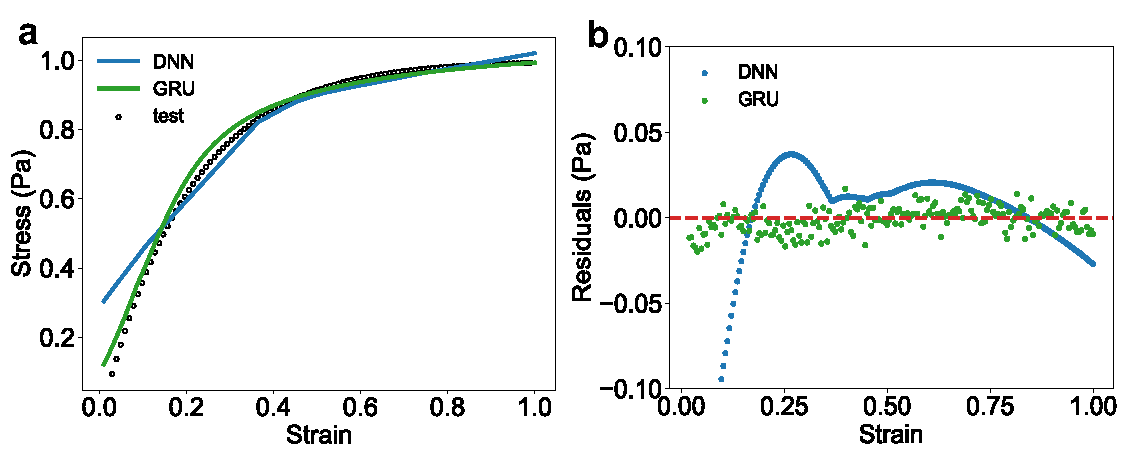
\includegraphics[width=0.8\textwidth]{Fig/maxwell_linear_test.pdf}
  \FigureBicaption{\label{maxwell_linear}GRU算法和DNN算法在Maxwell模型线性协议测试集上的预测效果对比示意图:(a)GRU和DNN在测试集上的预测值与真实值的应力-应变曲线(Lissajous曲线);(b)GRU和DNN在测试集上的预测值残差图}{Comparison of prediction performance between GRU and DNN algorithms on Maxwell model linear protocol test set: (a) Stress-strain curves (Lissajous curves) of predicted vs. true values for GRU and DNN on test set; (b) Residual plots of predicted values for GRU and DNN on test set}
\end{figure}
为了验证GRU算法在不同形式的应变历史下的泛化预测效果,本节使用交变应变协议生成的数据作为训练集,线性应变协议生成的数据作为测试集。分别使用了GRU和DNN进行训练,并在测试集上进行验证,测试结果如图\ref{maxwell_linear}、图\ref{maxwell_linear_metric}所示。
\begin{figure}[htbp]
  \centering
  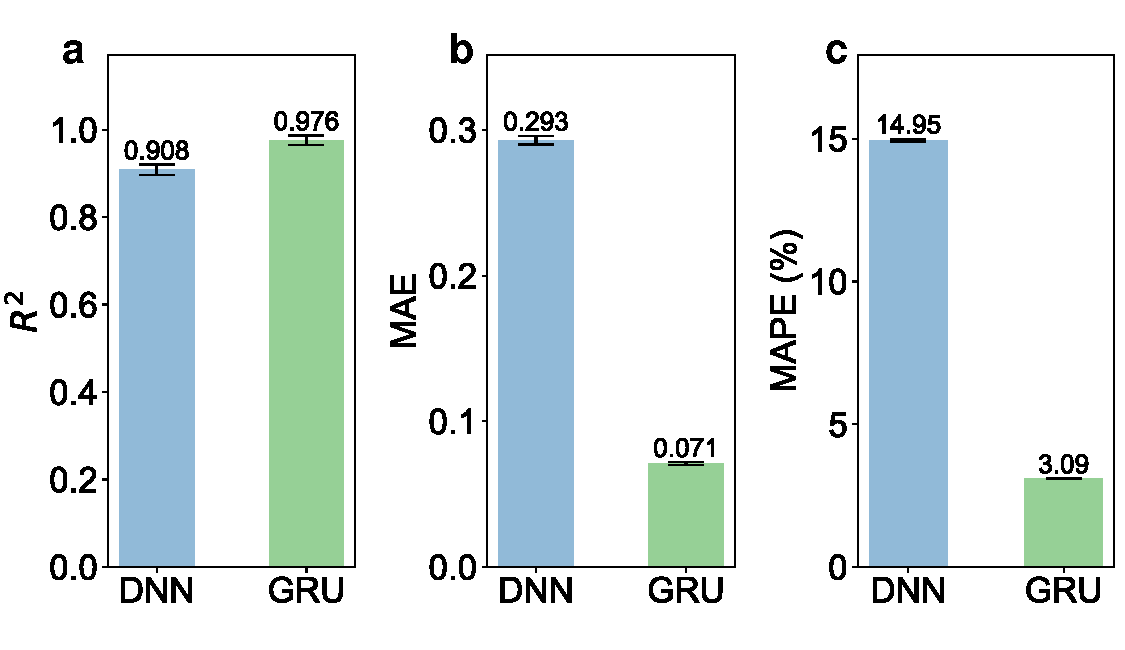
\includegraphics[width=0.8\textwidth]{Fig/maxwell_linear_metric.pdf}
  \FigureBicaption{\label{maxwell_linear_metric}GRU算法和DNN算法在Maxwell模型线性协议测试集上的预测指标对比图:(a)GRU和DNN在测试集上的R$^2$指标图;(b)GRU和DNN在测试集上的MAE指标图;(c)GRU和DNN在测试集上的MAPE指标图}{Comparison schematic of the prediction performance of the GRU algorithm and the DNN algorithm on the Maxwell model linear protocol test set: (a) R$^2$ metric plots on the test set for GRU and DNN; (b) MAE metric plots on the test set for GRU and DNN; (c) MAPE metric plots on the test set for GRU and DNN}
\end{figure}
图\ref{maxwell_linear}(a)为两种不同算法预测模型在测试集上的真实值-预测值的Lissajous曲线,图中可以看到GRU算法的预测值的Lissajous曲线与真实值曲线接近,在小应变时有一定偏差,这可能源于门控单元对初始状态记忆单元的权重初始化敏感性问题。而DNN算法的预测值的Lissajous曲线与真实的曲线相比GRU偏差更大,在小应变时,预测值与真实值有较大的偏差。

图\ref{maxwell_linear}(b)为两种算法预测模型的测试集残差图,从图中可以看到DNN算法的残差在初始时相比GRU更为偏离零刻度线,GRU的残差图残差点相对均匀地分布在零刻度线两侧,总体分布效果明显优于DNN的对应残差。这说明GRU捕捉到了训练数据的较完整的特征,且预测偏差较小。综合真实值-预测值曲线和残差图,可以定性分析出GRU的预测效果更为优秀。

接下来,本节计算两种算法的测试集预测指标,绘制指标对比图\ref{maxwell_linear_metric}。图\ref{maxwell_linear_metric}(a)显示,GRU的R$^2$值为0.976,接近1,证明GRU的预测效果十分优秀,而DNN的R$^2$值为0.908,略低于GRU,但是也高于0.9,属于非常出色的指标。仅从R$^2$指标来看,GRU预测效果优于DNN,但是优势不明显。从图\ref{maxwell_linear_metric}(b-c)看,GRU预测结果的MAE值为0.071,而DNN的预测结果的MAE值为0.293,GRU在绝对误差上仅为DNN的四分之一,优势显著。GRU预测结果的MAPE值为3.09,仅为DNN预测结果的MAPE值14.95的五分之一左右。这定量说明GRU的预测结果误差远小于DNN的预测结果误差,GRU在此项任务上预测泛化效果更好。这里的训练时间对比与上一节的交变协议预测交变协议一致,同图\ref{maxwell_sin_metric}(d)所示。


综合各项分析数据来看,当训练数据和测试数据为不同类型应变变化过程时,GRU算法展现出了显著的优势,尤其是在学习Maxwell模型数据的内在特征方面。Maxwell模型作为一种经典的粘弹性模型,其核心在于描述材料在应力作用下的时间依赖性响应。GRU算法可以仅通过学习交变应变的训练数据,就能够很好地预测线性应变的测试数据。这是因为GRU算法能够有效地从交变应变数据中提取出关键的时间依赖性特征,并将其应用于线性应变的预测中。
\subsubsection{不同时间步的预测效果对比}
\begin{figure}[htbp]
  \centering
  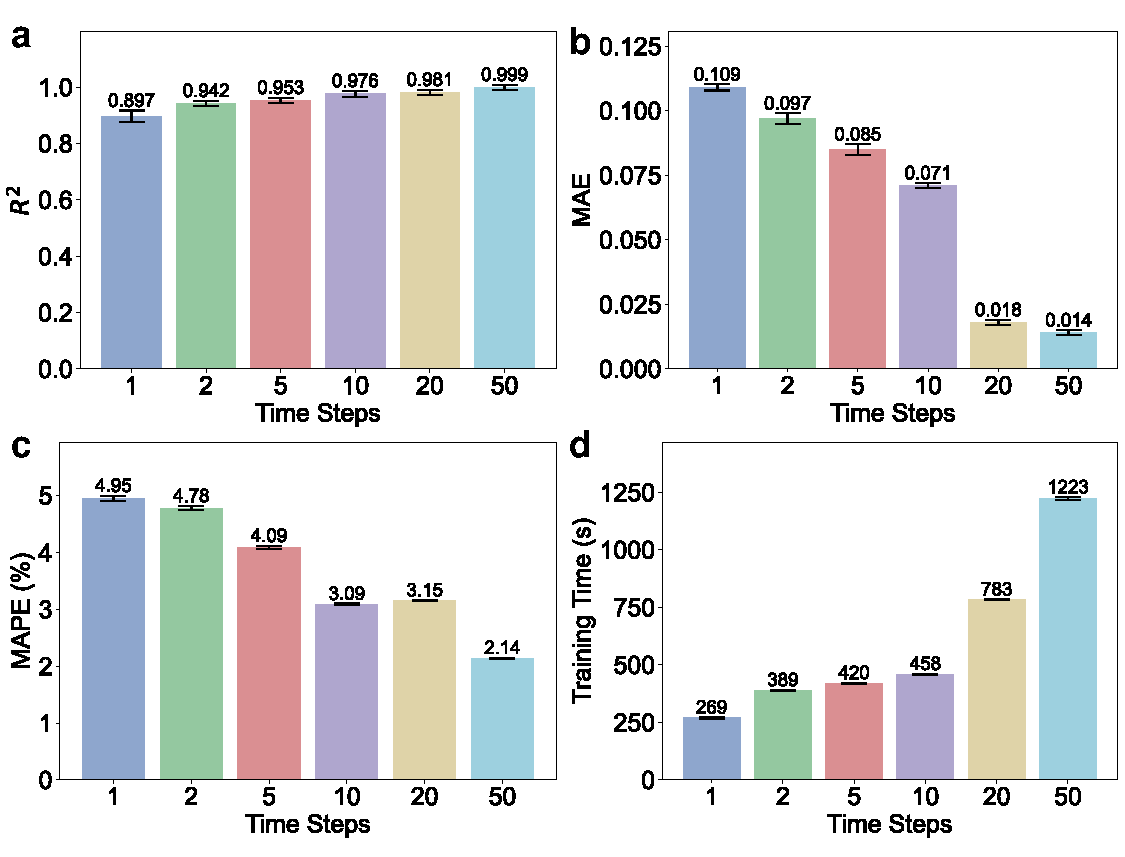
\includegraphics[width=0.8\textwidth]{Fig/Maxwell_timesteps_metrics.pdf}
  \FigureBicaption{\label{maxwell_timesteps_metrics}GRU算法在Maxwell模型不同时间步下的预测效果对比图:(a)GRU在不同时间步下的R$^2$指标图;(b)GRU在不同时间步下的MAE指标图;(c)GRU在不同时间步下的MAPE指标图;(d)GRU在不同时间步下的训练时间指标图}{Comparison of prediction performance of the GRU algorithm on the Maxwell model with different time steps: (a) R$^2$ metric plots with different time steps; (b) MAE metric plots with different time steps; (c) MAPE metric plots with different time steps; (d) Training Time metric plots with different time steps}
\end{figure}
对于GRU这类循环神经网络来说,网络架构的时间步数(序列长度)是非常重要的超参数。较大的时间步可以使模型在每个时间步上处理更多的信息,有助于捕捉长期依赖关系,但是可能导致模型学习到数据中的噪声,而不是其潜在的结构,从而导致过拟合。较小的时间步较小的时间步可以更细致地捕捉序列中的短期变化和细节信息,有助于模型更好地理解数据的短期动态特征,可能导致模型过于关注噪声,而忽略重要的长期依赖关系,从而导致欠拟合。本节研究了不同时间步下训练的模型在测试集上的预测效果。如图\ref{maxwell_timesteps_metrics}所示。由图可见,预测模型R$^2$值随着时间步的增加而增加,但是幅度较小。MAE值和MAPE值随时间步的增加而减少,说明随着时间步的增加,模型的预测效果变的更好,时间步小于10时,这种误差减小的趋势较明显,时间步大于20时,MAE值下降幅度变小,时间步大于10,MAPE值下降幅度变小。这说明模型的优化指标上升存在阈值,这是因为GRU算法在较长序列中容易遗忘丢失信息,对于时间序列的处理长度有一定限制。而随着时间步的增加,当时间步大于20后,模型的训练时间急剧增加,训练成本陡增。

本节分析针对此项任务,最佳时间步在10-20之间,MAE值和MAPE值开始下降到阈值,且训练时间还未显著增加。


% Doi-Edwards模型建模
\subsection{Doi-Edwards模型建模}
\subsubsection{数值模拟数据}
\begin{figure}[htbp]
  \centering
  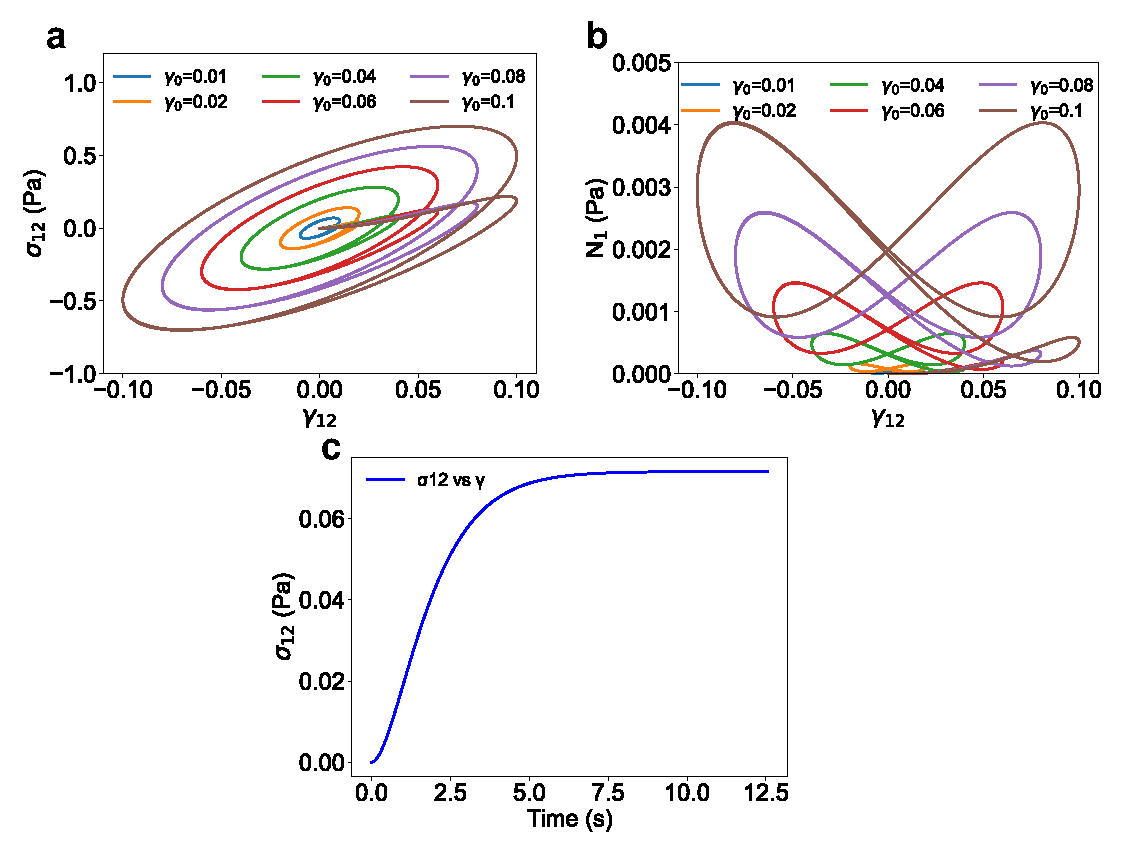
\includegraphics[width=0.8\textwidth]{Fig/doi-edwards-moni.pdf}
  \FigureBicaption{\label{doi-edwards-moni}Doi-Edwards模型模拟数据:(a)不同应变振幅下的剪切应力应变Lissajous曲线;(b)不同应变振幅下的第一法向应力差($N_1$)的Lissajous曲线;(c)线性应变协议下的应力-时间曲线}{Doi-Edwards model simulation data: (a) Lissajous curves of shear stress-strain under different strain amplitudes; (b) Lissajous curves of first normal stress difference ($N_1$); (c) Stress-time curves under linear strain protocol}
\end{figure}
本节使用Python的scipy.integrate库对Doi-Edwards模型进行数值积分模拟。模拟结果如图\ref{doi-edwards-moni}所示。图\ref{doi-edwards-moni}(a)为不同应变振幅模拟的剪切应力应变Lissajous曲线,曲线呈现标准的椭圆形状,符合Doi-Edwards模型在小应变下的假设。图\ref{doi-edwards-moni}(b)为模拟的第一法向应力差($N_1$)的Lissajous曲线,曲线具有振幅依赖性,且为滞回曲线,与文献中的Doi-Edwards模型一致。图\ref{doi-edwards-moni}(c)为线性应变协议下的应力-时间曲线,可以看到随着应变加载,应力一开始为近似的线性增加,后逐渐趋向平台值,这个结果符合预期。综上本节模拟的数据可以认为符合Doi-Edwards模型,可以用于后续实验。

\subsubsection{交变协议预测交变协议效果验证}
\begin{figure}[htbp]
  \centering
  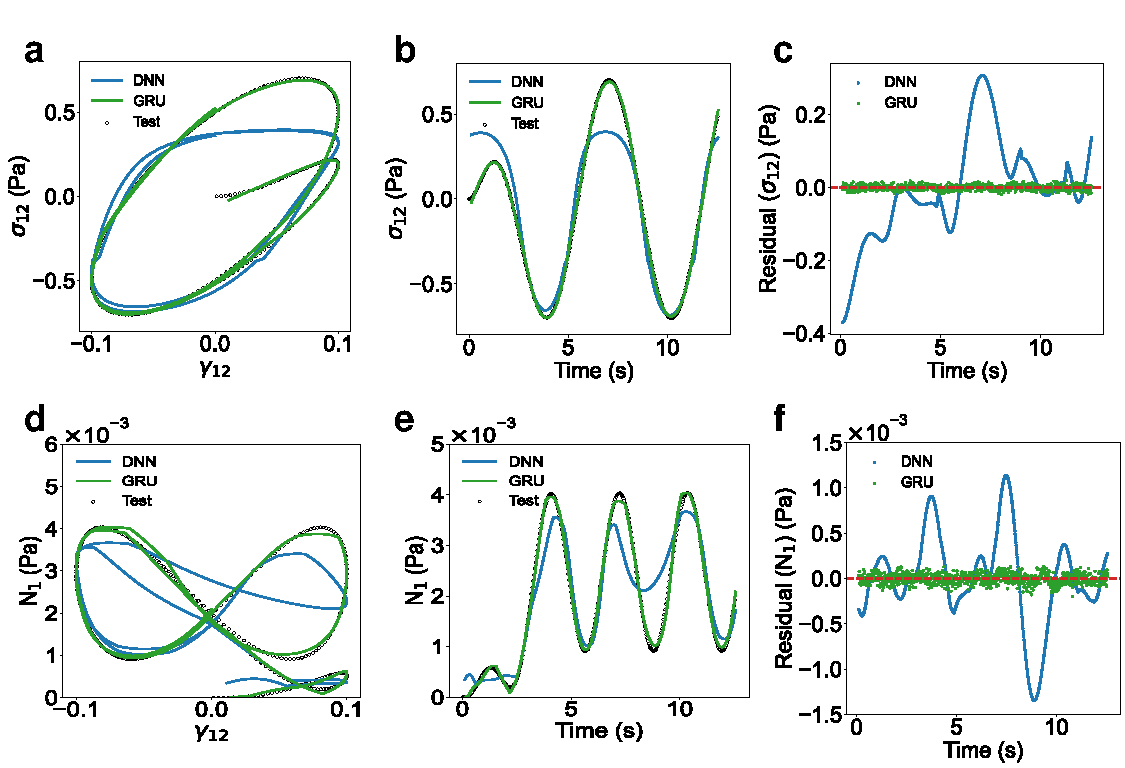
\includegraphics[width=0.8\textwidth]{Fig/doi-edwards-sin.pdf}
  \FigureBicaption{\label{doi-edwards-sin}GRU算法和DNN算法在Doi-Edwards模型交变协议测试集上的预测效果对比示意图:(a)GRU和DNN在测试集上的预测值与真实值的剪切应力-应变曲线(Lissajous曲线);(b)GRU和DNN在测试集上的预测值与真实值的时间-应力曲线;(c)GRU和DNN在测试集上剪切应力的预测值残差图;(d)GRU和DNN在测试集上的预测值与真实值的第一法向应力差($N_1$)的Lissajous曲线;(e)GRU和DNN在测试集上的预测值与真实值的时间-第一法向应力差曲线;(f)GRU和DNN在测试集上的第一法向应力差预测值残差图}{Comparison schematic of the prediction performance of the GRU algorithm and the DNN algorithm on the Doi-Edwards model alternating protocol test set: (a) Shear stress-strain curves (Lissajous curves) of predicted vs. true values for GRU and DNN on test set; (b) Time-stress curves of predicted vs. true values for GRU and DNN on test set; (c) Residual plots of shear stress predicted values for GRU and DNN on test set; (d) First normal stress difference ($N_1$) Lissajous curves of predicted vs. true values for GRU and DNN on test set; (e) Time-first normal stress difference curves of predicted vs. true values for GRU and DNN on test set; (f) Residual plots of first normal stress difference predicted values for GRU and DNN on test set}
\end{figure}
\begin{figure}[htbp]
  \centering
  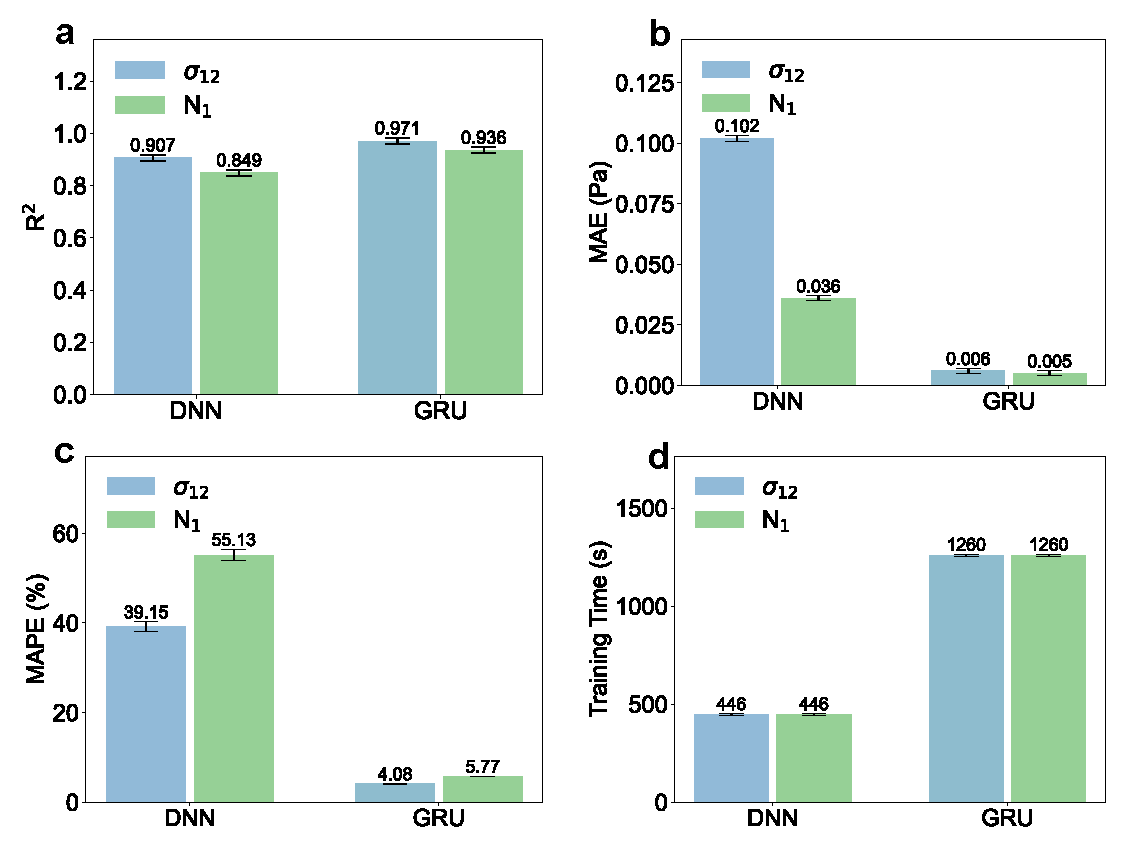
\includegraphics[width=0.8\textwidth]{Fig/doi-edwards-sin-metrics.pdf}
  \FigureBicaption{\label{doi-edwards-sin-metric}GRU算法和DNN算法在Doi-Edwards模型交变协议测试集上的预测指标对比图:(a)GRU和DNN在测试集上的R$^2$指标图;(b)GRU和DNN在测试集上的MAE指标图;(c)GRU和DNN在测试集上的MAPE指标图;(d)GRU和DNN在测试集上的训练时间指标图}{Comparison schematic of the prediction performance of the GRU algorithm and the DNN algorithm on the Doi-Edwards model alternating protocol test set: (a) R$^2$ metric plots on the test set for GRU and DNN; (b) MAE metric plots on the test set for GRU and DNN; (c) MAPE metric plots on the test set for GRU and DNN; (d) Training Time metric plots on the test set for GRU and DNN}
\end{figure}
为了验证GRU算法在Doi-Edwards模型本构方程数据中的预测效果,本节使用交变应变协议生成的数据作为训练集,交变应变协议生成的数据作为测试集。分别使用了GRU和DNN进行训练,并在测试集上进行验证,测试结果如图\ref{doi-edwards-sin}、图\ref{doi-edwards-sin-metric}所示。

图\ref{doi-edwards-sin}(a-c)为两种不同算法构建的预测模型预测的剪切应力($\sigma_{12}$)的Lissajous曲线、时间-应力曲线、残差图,(d-f)为预测的第一法向应力差($N_1$)的Lissajous曲线、时间-应力曲线、残差图。
图a和图b可以看出GRU算法的预测的$\sigma_{12}$值与真实的$\sigma_{12}$接近,曲线拟合较好。而DNN算法的预测值在某些区域存在较大误差,例如在应变变化的初始和$5\sim10$ s之间,DNN存在较大误差。图c的残差图则显示,GRU算法预测值与真实值的残差紧贴零刻度线,呈现无序离散的分布状态,而DNN算法预测值和真实值的残差呈现明显的曲线规律,且与零刻度线性距离偏差较大,残差分布区间远远大于GRU部分。残差图的结果表明对于GRU成功地学习到了训练数据中的各项特征,复杂的非线性关系,且不存在明显周期性,总体残差较小,而DNN存在特征未能完全学习的问题,拟合效果较差,未能很好地捕捉到训练数据的特征。从图d、图e和图f的$N_1$的预测效果图来看,$N_1$与$\sigma_{12}$的结果类似,均是GRU的预测效果要由于DNN,而对比GRU预测的$N_1$值和$\sigma_{12}$值,则是$\sigma_{12}$值的预测效果会更好,这可能是因为$\sigma_{12}$与输入的剪切速率特征$\dot{\gamma_{12}}$之间的函数关系更为简单,且更加符合时间叠加原理,所以GRU可以更好地捕捉其时间依赖性和内在联系。


之后本节分别对两种不同算法在$\sigma_{12}$和$N_1$上的预测效果做了定量分析,指标图如图\ref{doi-edwards-sin-metric}所示。在R$^2$指标上,GRU在$\sigma_{12}$和$N_1$的预测指标均优于DNN,而同种算法下$\sigma_{12}$的R$^2$值要高于$N_1$,显示$\sigma_{12}$的预测效果更好。在MAE指标上,DNN的$\sigma_{12}$和$N_1$的MAE值均远高于GRU,说明GRU的预测误差远小于DNN。MAPE指标与MAE指标的对比基本一致,都是GRU的预测误差小于DNN。但是同种算法下$\sigma_{12}$的MAE值高于$N_1$,但是MAPE值反之,这是因为MAE值强调的是绝对值比较,受到真实数据本身尺度的影响,因此比较同种算法下$\sigma_{12}$和$N_1$的预测效果应当以去除了数据尺度影响的MAPE值来判定,而MAPE值的结论表明同种算法下$\sigma_{12}$值的预测效果相比$N_1$更好,这与R$^2$的分析和图\ref{doi-edwards-sin}的定性分析一致,这也是后续可以优化的方向之一。最后,从图\ref{doi-edwards-sin-metric}(d)来看,GRU在此项任务上的训练时间为DNN的3倍左右,符合更高成本的预期。

综合各项分析数据来看,当训练数据和测试数据为同类型应变变化过程(都为交变应变)时,GRU算法可以更好的学习到Doi-Edwards模型数据的内在特征,包括周期性响应,黏弹性,时间依赖性响应。从定性与定量分析结果看,GRU算法的预测泛化效果在此项任务上明显优于DNN,在计算资源足够时,GRU算法相比DNN性能更佳,而在同种算法下$\sigma_{12}$的预测效果优于$N_1$。
\subsubsection{交变预测稳态协议效果验证}
\begin{figure}[htbp]
  \centering
  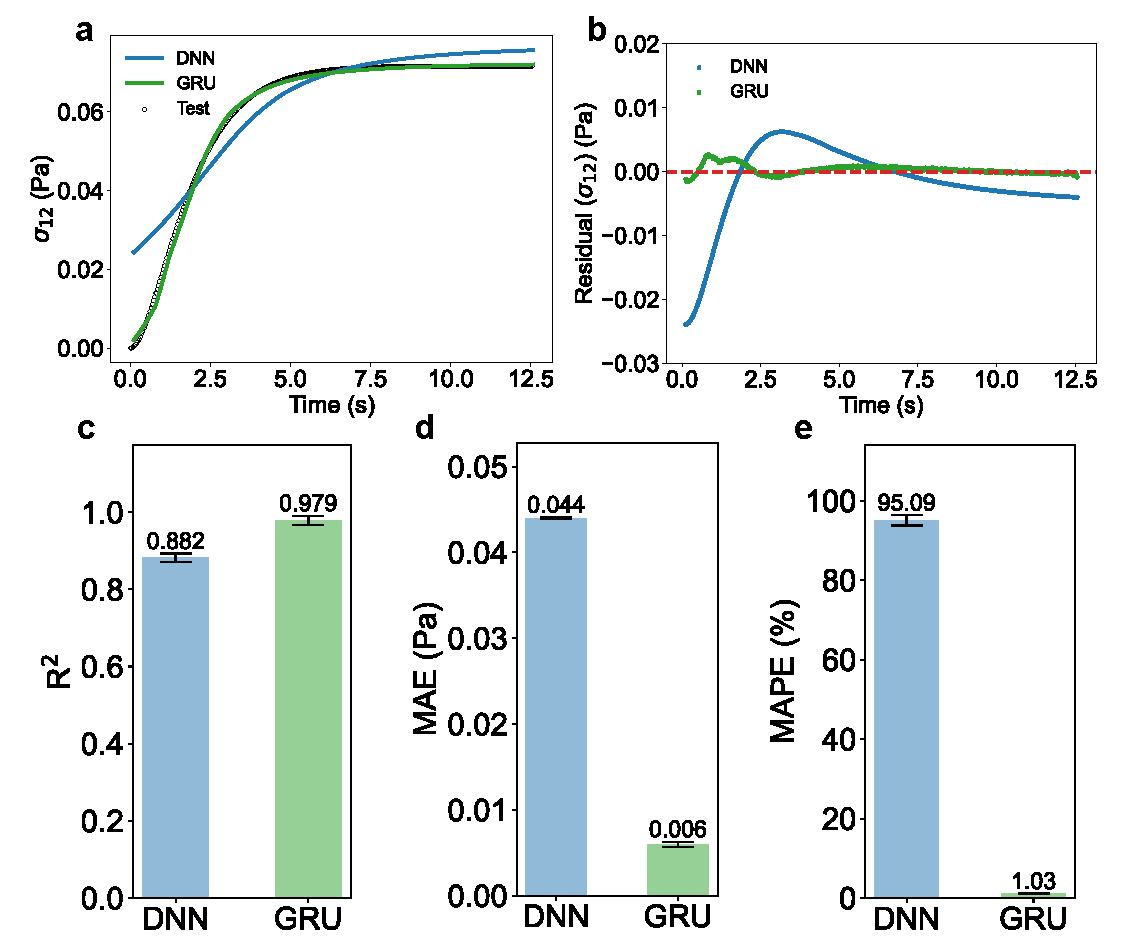
\includegraphics[width=0.8\textwidth]{Fig/doi-edwards-linear.pdf}
  \FigureBicaption{\label{doi-edwards-linear}GRU算法和DNN算法在Doi-Edwards模型线性协议测试集上的预测效果对比示意图:(a)GRU和DNN在测试集上的预测值与真实值的剪切应力-应变曲线(Lissajous曲线);(b)GRU和DNN在测试集上的预测值残差图}{Comparison schematic of the prediction performance of the GRU algorithm and the DNN algorithm on the Doi-Edwards model linear protocol test set: (a) Shear stress-strain curves (Lissajous curves) of predicted vs. true values for GRU and DNN on test set; (b) Residual plots of predicted values for GRU and DNN on test set}
\end{figure}
\begin{figure}[htbp]
  \centering
  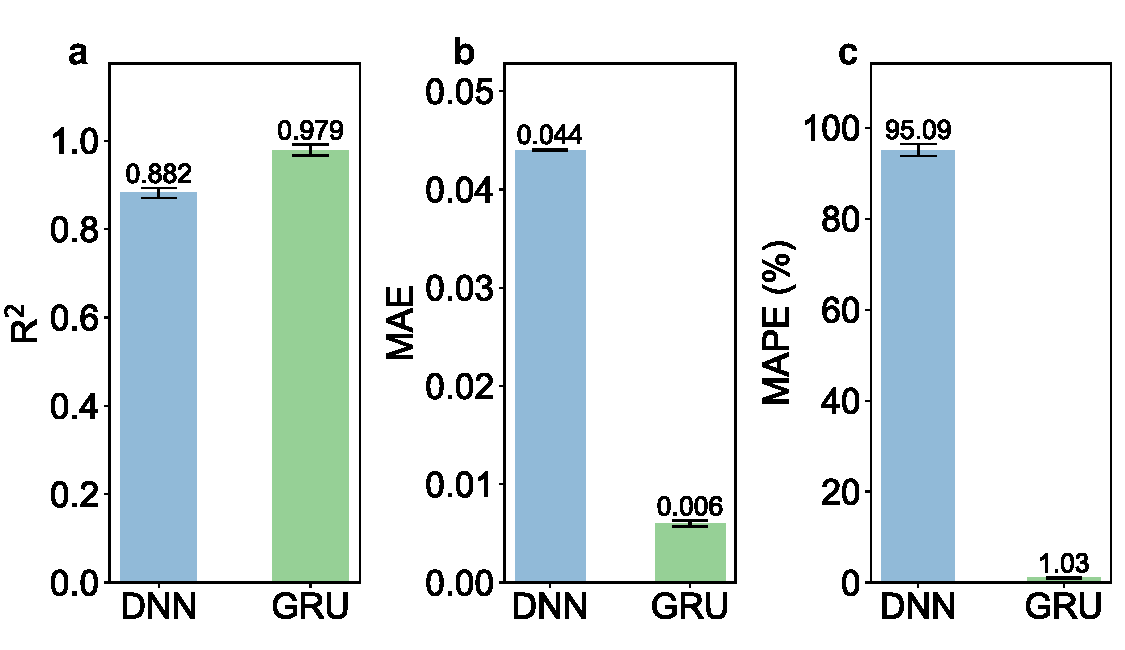
\includegraphics[width=0.8\textwidth]{Fig/doi-edwards-linear-metrics.pdf}
  \FigureBicaption{\label{doi-edwards-linear-metrics}GRU算法和DNN算法在Doi-Edwards模型线性协议测试集上的预测效果对比示意图:(a)GRU和DNN在测试集上的R$^2$指标图;(b)GRU和DNN在测试集上的MAE指标图;(c)GRU和DNN在测试集上的MAPE指标图}{Comparison schematic of the prediction performance of the GRU algorithm and the DNN algorithm on the Doi-Edwards model linear protocol test set: (a) R$^2$ metric plots on the test set for GRU and DNN; (b) MAE metric plots on the test set for GRU and DNN; (c) MAPE metric plots on the test set for GRU and DNN}
\end{figure}
为了验证GRU算法在不同形式的应变历史下对于Doi-Edwards模型泛化预测效果,本节使用交变应变协议生成的数据作为训练集,线性应变协议生成的数据作为测试集。分别使用了GRU和DNN进行训练,并在测试集上进行验证,测试结果如图\ref{doi-edwards-linear}、图\ref{doi-edwards-linear-metrics}所示。

图\ref{doi-edwards-linear}(a)为两种不同算法预测模型在测试集上的真实值-预测值曲线,图中可以看到GRU算法的预测值的曲线与真实值曲线接近,无较明显的偏差区间,而DNN算法的预测值的曲线与真实的曲线存在明显的偏差。在应变加载初始和结束时,DNN算法的预测值相比真实值偏大,而应变加载$2\sim6$ s的中间阶段,DNN算法的预测值又偏小,总体来看仅在大致趋势上符合真实值曲线。

图\ref{doi-edwards-linear}(b)展示了两种算法在测试集上的残差图。从图中可以明显看出,DNN算法的预测值与真实值之间的残差分布并不均匀,整体呈现出较为清晰的曲线趋势,尤其是在第3 s附近出现了显著的峰值。这表明DNN未能充分捕捉到训练数据中的关键特征,导致其在测试集上的表现不佳。相比之下,GRU算法的残差图则呈现出无序分布,残差点均匀地分布在零刻度线两侧,且残差值普遍小于DNN。这说明GRU能够更好地捕捉到训练数据中的特征,预测偏差也更小。综合真实值与预测值的曲线以及残差图的分析,可以定性地得出结论:GRU的预测效果优于DNN。

接下来,本节对两种算法在测试集上的预测性能指标进行了详细计算,并绘制了相应的指标对比图,如图\ref{doi-edwards-linear-metrics}所示。从图\ref{doi-edwards-linear-metrics}(a)中可以看出,GRU算法的 R$^2$值达到了0.979,这一结果充分证明了GRU在预测任务中的卓越表现。相比之下,DNN算法的 R$^2$值仅为0.882,明显低于GRU,这表明在 R$^2$指标的评估中,GRU的表现更为出色。进一步观察图\ref{doi-edwards-linear-metrics}(b-c),可以发现GRU预测结果的MAE值为0.006,而DNN的MAE值则高达0.044。这意味着GRU在绝对误差方面的表现仅为DNN的七分之一,优势极为显著。此外,GRU预测结果的MAPE值为1.03,而DNN的MAPE值则为95.09。这些定量数据充分说明了GRU的预测结果误差远小于DNN,从而证明了GRU在该任务上的预测泛化能力更强。
至于训练时间的对比,与上一节中交变协议预测交变协议的情况一致,具体可参考图\ref{doi-edwards-sin-metric}(d)所示。

从整体分析数据来看,当训练数据与测试数据涉及不同类型的应变变化过程时,GRU算法在学习Doi-Edwards模型数据的内在特性方面有显著优势。这主要归因于GRU算法能够高效地从交变应变数据中提取关键的时间依赖特征,并将其成功应用于线性应变的预测之中。

\subsubsection{不同时间步的预测效果对比}

为了探究在Doi-Edwards模型上GRU算法的最佳时间步,本节研究了不同时间步下训练的模型在测试集上的预测效果,如图\ref{doi-edwards-timesteps-metrics}所示。由图可见,预测模型R$^2$值在时间步小于40时随着时间步的增加而增加,在时间步大于40后反而略有下降。MAE值和MAPE值在时间步小于40时随时间步的增加而减少,时间步为40的值只有不到时间步为20的值的十分之一,显著下降,而时间步大于40后,MAE值和MAPE值则趋于稳定。这说明对于本项任务,时间步为40左右时,恰好可以开始获得不错的预测效果,而从训练成本来看,训练时间是随着时间步设置增加而单调增的,所以综合看来,时间步为40左右时,性价比最高。
\begin{figure}[H]
  \centering
  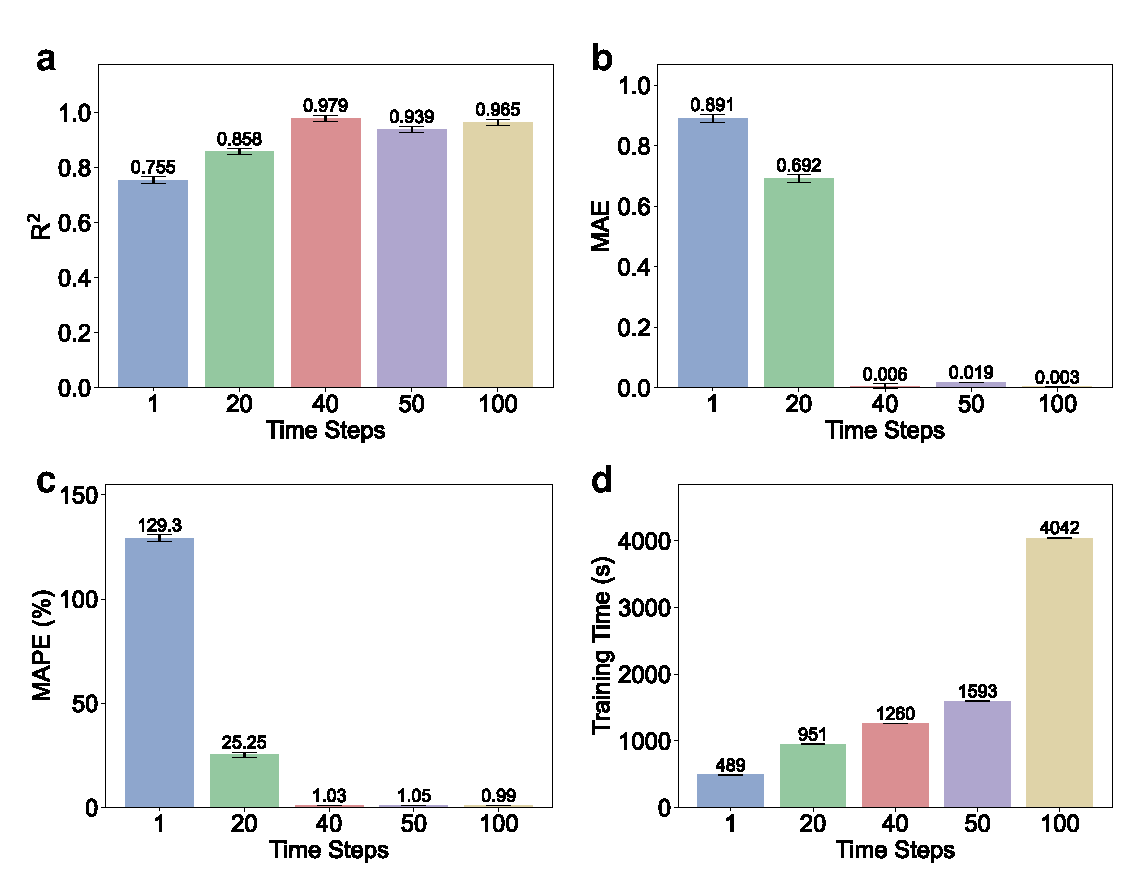
\includegraphics[width=0.8\textwidth]{Fig/doi-edwards-timesteps-metrics.pdf}
  \FigureBicaption{\label{doi-edwards-timesteps-metrics}GRU算法和DNN算法在Doi-Edwards模型不同时间步长下的预测指标对比图:(a)GRU和DNN在不同时间步下的R$^2$指标图;(b)GRU和DNN在不同时间步下的MAE指标图;(c)GRU和DNN在不同时间步下的MAPE指标图;(d)GRU和DNN在不同时间步下的训练时间指标图}{Comparison schematic of the prediction performance of the GRU algorithm and the DNN algorithm under different time steps of the Doi-Edwards model: (a) R$^2$ metric plots under different time steps for GRU and DNN; (b) MAE metric plots under different time steps for GRU and DNN; (c) MAPE metric plots under different time steps for GRU and DNN; (d) Training Time metric plots under different time steps for GRU and DNN}
\end{figure}
\subsection{Giesekus模型建模}
\subsubsection{振荡剪切预测振荡剪切}
本节通过数值模拟不同应变幅值和频率的Giesekus模型振荡剪切数据,将其输入PI-GRU模型进行训练,并评估模型对未知振荡剪切数据的预测能力。图\ref{pigru-giesekus-sin}展示了PI-GRU、MLP和GRU模型(不含物理约束损失)在测试集上的预测结果与真实数据对比,图\ref{pigru-giesekus-sin-metrics}则展示了相应的评价指标。
\begin{figure}
  \centering
  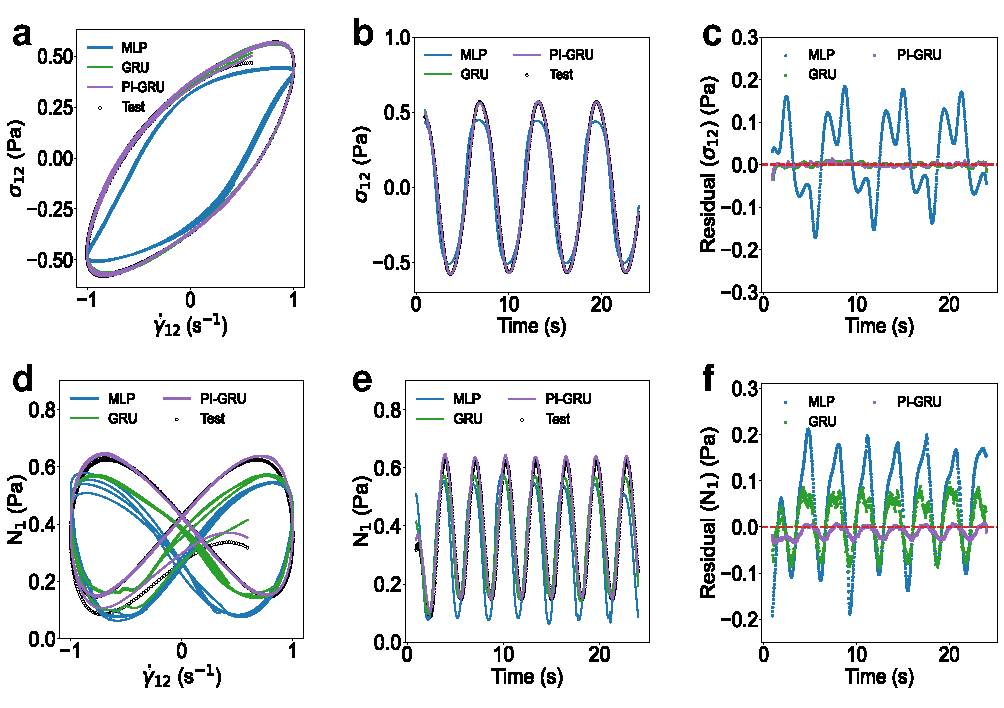
\includegraphics[width=0.9\textwidth]{Fig/pigru-giesekus-sin.pdf}
  \FigureBicaption  {\label{pigru-giesekus-sin}Giesekus数值模拟振荡剪切数据(LAOS)测试集上PI-GRU、MLP和GRU模型的预测结果与真实数据对比,这里训练数据与测试数据均为大振幅振荡剪切数据:(a)剪切应力$\sigma_{12}$真实值与模型预测值Lissajous曲线;(b)剪切应力$\sigma_{12}$真实值与模型预测值的时间-应力曲线;(c)剪切应力$\sigma_{12}$真实值与模型预测值残差图;(d)第一法向应力差N$_1$真实值与模型预测值Lissajous曲线;(e)第一法向应力差N$_1$真实值与模型预测值的时间-应力曲线;(f)第一法向应力差N$_1$真实值与模型预测值残差图}{Comparison schematic of the prediction results of the PI-GRU, MLP, and GRU models on the Giesekus numerical simulation oscillatory shear data test set: (a) Lissajous curve of the true value and predicted value of the shear stress $\sigma_{12}$ for the GRU model; (b) time-stress curve of the true value and predicted value of the shear stress $\sigma_{12}$ for the GRU model; (c) residual plot of the true value and predicted value of the shear stress $\sigma_{12}$ for the GRU model; (d) Lissajous curve of the true value and predicted value of the first normal stress difference N$_1$ for the GRU model; (e) time-stress curve of the true value and predicted value of the first normal stress difference N$_1$ for the GRU model; (f) residual plot of the true value and predicted value of the first normal stress difference N$_1$ for the GRU model}
\end{figure}
本节中PI-GRU模型采用上对流Maxwell模型(UCM)作为物理约束,其表达式如公式\ref{eq:ucm}所示。UCM可视为Giesekus模型的简化形式,省略了流动指数$\alpha$项,因此理论上UCM只能部分捕捉Giesekus模型的特征。
\begin{equation}
  \boldsymbol{\sigma} + \lambda \stackrel{\triangledown}{\boldsymbol{\sigma}} = \eta \dot{\boldsymbol{\gamma}} \label{eq:ucm}
\end{equation}

\begin{figure}
  \centering
  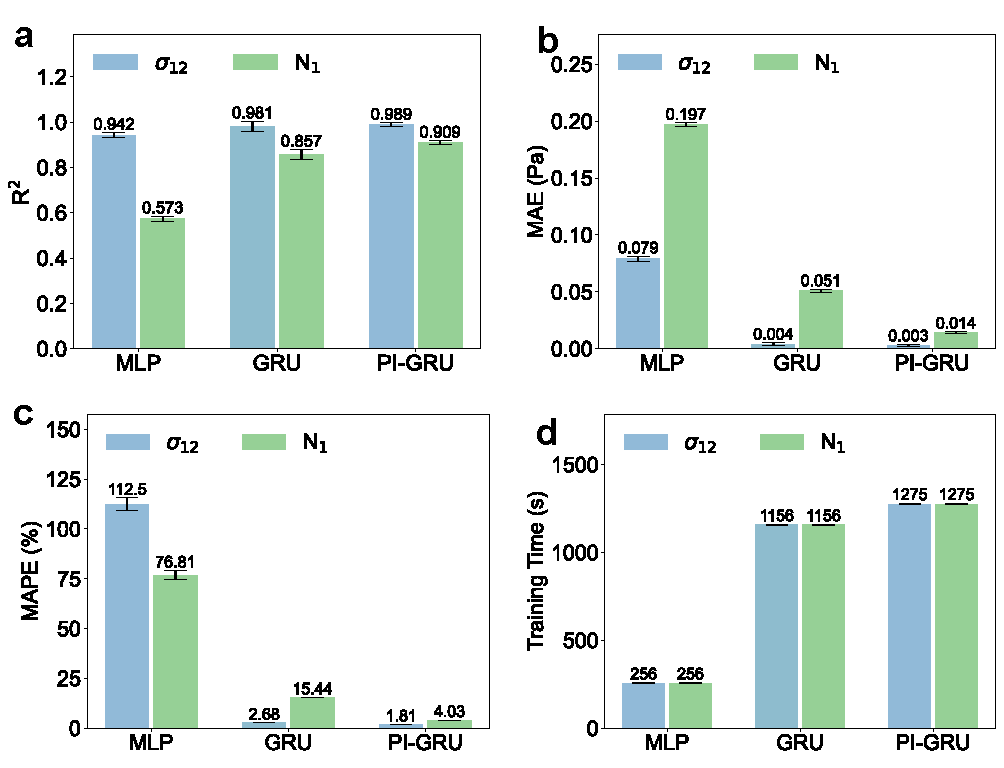
\includegraphics[width=0.9\textwidth]{Fig/pigru-giesekus-sin-metrics.pdf}
  \FigureBicaption{\label{pigru-giesekus-sin-metrics}Giesekus数值模拟振荡剪切数据测试集上PI-GRU、MLP和GRU模型的评价指标:(a)R$^2$值;(b)MAE值;(c)MAPE值;(c)训练时间}{Comparison schematic of the evaluation metrics of the PI-GRU, MLP, and GRU models on the Giesekus numerical simulation oscillatory shear data test set: (a) R$^2$ value; (b) MAE value; (c) MAPE value; (d) training time}
\end{figure}
结果表明,作为前馈神经网络的MLP模型在预测剪切应力($\sigma_{12}$)和第一法向应力差($N_1$)时表现最差,这符合前馈神经网络难以有效捕捉长序列时间依赖关系的预期。

GRU模型在处理时间依赖关系方面表现出色,图\ref{pigru-giesekus-sin}(a,b)中其预测曲线与真实值高度吻合,明显优于MLP模型。图\ref{pigru-giesekus-sin}c的残差分析进一步证实MLP的残差呈现明显的趋势性偏差,而GRU的残差则均匀分布在零线附近,表明其具有更强的特征学习能力。图\ref{pigru-giesekus-sin-metrics}(a,b,c)

值得指出的是,在剪切应力预测任务中,引入UCM物理约束的PI-GRU模型(MAPE=1.81\%)相比GRU模型(MAPE=2.68\%)提升不显著。然而,在第一法向应力差$N_1$的预测中,PI-GRU模型(MAPE=4.03\%)明显优于GRU(MAPE=15.44\%)和MLP(MAPE=76.81\%)。

第一法向应力差预测难度高于剪切应力的原因在于$N_1$是应力张量对角元素的差值($\sigma_{11}-\sigma_{22}$),其计算涉及多个应力分量,误差容易累积。其次,$N_1$对材料非线性响应更敏感,在大应变下变化更为剧烈,需要模型具备更强的非线性特征提取能力。UCM模型虽然简化,但仍包含了应力张量的上对流导数项,能够部分捕捉材料在剪切流动中的非线性行为,特别是法向应力差的产生机制。这种物理约束引导模型学习符合流变学基本原理的特征表示,从而在预测具有挑战性的$N_1$时表现出更强的泛化能力。

综上所述,将传统MLP结构升级为具有记忆能力的GRU结构,并结合物理约束损失函数,能够显著增强模型捕捉黏弹性材料时间依赖特性的能力。这种结构优化使得模型在处理复杂非线性流变学数据时表现出优越的预测精度,特别是在法向应力差等难以预测的参数上。值得注意的是,PI-GRU模型由于其循环神经网络的内在特性,计算复杂度较高,导致训练时间(图\ref{pigru-giesekus-sin-metrics}d所示)显著长于MLP结构,这一现象在本研究的所有实验任务中均有体现。尽管如此,本任务中1275秒的训练时间仍处于可接受范围内。PI-GRU模型为复杂流变学本构关系的高效建模提供了新思路,原本需要大量不同振荡条件的实验数据才能描述的本构关系,或许可以使用有限的数据建立模型,再去泛化到未知实验条件的数据,从而减少实验成本并加速材料开发过程。
\subsubsection{振荡剪切预测稳态剪切}
当训练集与测试集都为正弦振荡剪切时,这种同分布测试无法有效验证模型是否真正建立了Giesekus模型的本构关系映射。Giesekus模型的核心特征在于其非线性应力响应特性,包括剪切稀化等特性。因此,本研究做了振荡剪切预测稳态剪切的实验来探究PI-GRU模型是否能够正确预测稳态剪切下的应力应变关系,真正重现Giesekus本构方程。图\ref{pigru-giesekus-linear}展示了PI-GRU模型在测试集上的预测结果与真实数据对比。
\begin{figure}
  \centering
  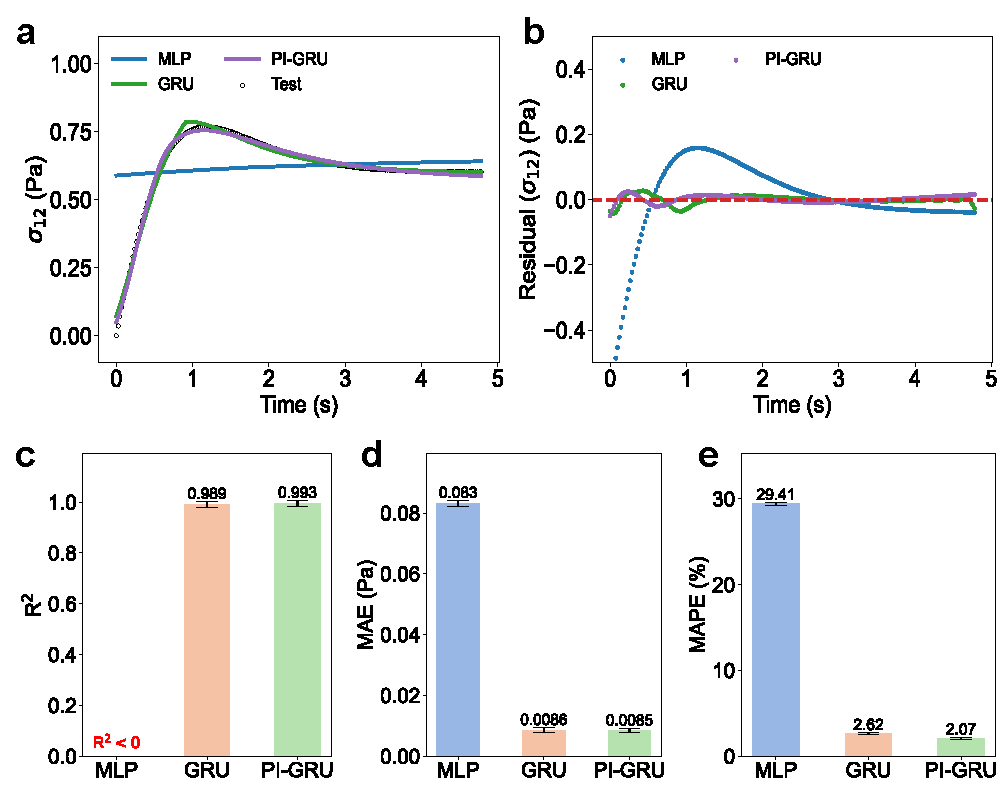
\includegraphics[width=0.9\textwidth]{Fig/pigru-giesekus-linear.pdf}
  \FigureBicaption{\label{pigru-giesekus-linear}Giesekus数值模拟稳态剪切数据测试集上PI-GRU、MLP和GRU模型的预测结果与真实数据对比,这里训练数据为大振幅振荡剪切(LAOS)数据,测试数据为稳态剪切数据:(a)剪切应力$\sigma_{12}$真实值与模型预测值的时间-应力曲线;(b)剪切应力$\sigma_{12}$真实值与模型预测值残差图;(c)R$^2$值;(d)MAE值;(e)MAPE值}{Comparison schematic of the prediction results of the PI-GRU, MLP, and GRU models on the Giesekus numerical simulation steady-state shear data test set: (a) time-stress curve of the true value and predicted value of the shear stress $\sigma_{12}$ for the GRU model; (b) residual plot of the true value and predicted value of the shear stress $\sigma_{12}$ for the GRU model; (c) R$^2$ value; (d) MAE value; (e) MAPE value}
  \label{pigru-giesekus-linear}
\end{figure}

可以看到面对不同应变协议的Giesekus测试数据,GRU和PI-GRU的预测效果明显优于MLP,从预测曲线(图\ref{pigru-giesekus-linear}a)和残差分析(图\ref{pigru-giesekus-linear}b)以及定量评估指标(图\ref{pigru-giesekus-linear}(c-e))来看,MLP完全无法从振荡剪切数据泛化稳态剪切数据,R$^2$值甚至出现了负数,这说明纯数据驱动的MLP模型无法理解Giesekus模型中的非线性特征。将神经网络结构改为GRU后,预测效果得到明显改善(R$^2$=0.989,MAE=0.0086,MAPE=2.62\%)。
PI-GRU模型表现出最佳的预测泛化效果,R$^2$值为0.993(>0.99),MAE指标再降低至0.0085,MAPE指标仅为2.07\%,这表明PI-GRU模型能够很好学习到Giesekus模型中的非线性特征,并能够从振荡剪切数据泛化到稳态剪切数据。图\ref{pigru-giesekus-linear}a显示Giesekus模型在稳态剪切下首先表现为弹性主导的应力增长响应,之后应力衰减对应剪切稀化现象,最后黏性主导下呈现平台,PI-GRU模型能够从振荡剪切数据中正确识别出这些Giesekus模型的特征,将相关的时间依赖性特征与非线性特征嵌入到模型的参数中,最后在稳态剪切下预测出与真实数据高度吻合的应力应变曲线。

这是一个有趣的发现,一般认为振荡剪切与稳态剪切在非线性区间是有差异的,前者通过动态加载揭示材料的弹性记忆、高阶谐波响应及非对称性,后者则侧重稳态流动下的黏性行为。然而,本研究结果表明,PI-GRU模型在振荡剪切数据上训练后,能够较准确预测稳态剪切下的应力应变关系,这意味着PI-GRU有着构建完备统一本构关系的能力,同时相对易获取的振荡剪切数据可以低成本去构建各种复杂工况,例如注塑成型、挤出成型大剪切形变下的本构关系。在此基础上,这套方法或可大幅缩短实验周期,指导黏弹性材料的配方优化与工艺参数选择,显著降低工业试错成本。

\subsubsection{线性预测非线性}
在流变学本构方程的研究中,非线性本构方程的数学建模和参数拟合难度往往远远大于线性本构方程,在实际的流变学测试中,能够获取非线性数据的大振幅剪切实验(LAOS)实验成本也远远高于小振幅剪切实验(SAOS)。因此,如果能够从线性的SAOS数据出发,探究出非线性区间的全部或部分本构关系,对是流变学家非常乐于见到的。本研究通过构建PI-GRU模型,做了这样的尝试:训练数据全部采用SAOS数据,测试数据全部采用LAOS数据,探究PI-GRU模型是否能够从线性区间的SAOS数据泛化到非线性区间的LAOS数据。
\begin{figure}
  \centering
  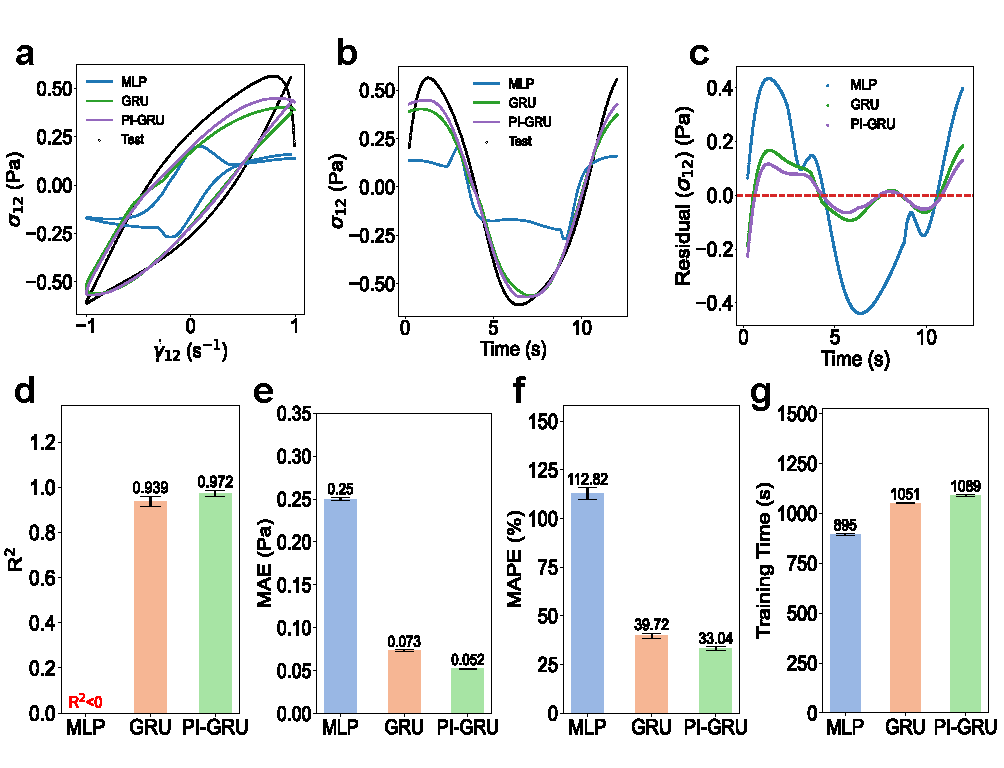
\includegraphics[width=0.9\textwidth]{Fig/giesekus-saos2laos.pdf}
  \FigureBicaption{\label{giesekus-saos2laos}Giesekus数值模拟线性SAOS数据预测非线性LAOS数据测试集上PI-GRU、MLP和GRU模型的预测结果与真实数据对比,这里训练数据为SAOS数据,测试数据为LAOS数据:(a)剪切应力$\sigma_{12}$真实值与模型预测值的Lissajous曲线;(b)剪切应力$\sigma_{12}$真实值与模型预测值的时间-应力曲线;(c)剪切应力$\sigma_{12}$真实值与模型预测值残差图;(d)R$^2$值;(e)MAE值;(f)MAPE值;(g)训练时间}{Comparison schematic of the prediction results of the PI-GRU, MLP, and GRU models on the Giesekus numerical simulation linear SAOS data prediction nonlinear LAOS data test set: (a) Lissajous curve of the true value and predicted value of the shear stress $\sigma_{12}$ for the GRU model; (b) time-stress curve of the true value and predicted value of the shear stress $\sigma_{12}$ for the GRU model; (c) residual plot of the true value and predicted value of the shear stress $\sigma_{12}$ for the GRU model; (d) R$^2$ value; (e) MAE value; (f) MAPE value; (g) training time}
  \label{giesekus-saos2laos}
\end{figure}

这里还是选取了MLP,GRU和PI-GRU模型进行对比,所使用的训练集全部都是SAOS数据,最终图\ref{giesekus-saos2laos}绘制的是LAOS测试集的对比图,可以发现MLP在预测LAOS数据时,预测曲线与真实曲线偏差较大,各指标表现较差(R$^2$<0,MAE=0.25,MAPE=112.82\%),GRU和PI-GRU模型在预测LAOS数据时,预测效果相对MLP得到一定提升,图\ref{giesekus-saos2laos}(a-c)可以定性看出不同模型之间的预测效果是:PI-GRU>GRU>MLP。
在定量指标方面,GRU的MAPE值为39.72\%,相比MLP的112.82\%降低了73.1\%,可以说得到了本质的优化,而PI-GRU模型在GRU的基础上,进一步引入了物理约束,MAPE值为33.04\%,相比GRU仅仅降低了6.68\%,说明物理约束对模型在此项任务上的提升有限。这里的结果可能是因为,训练数据中数据都是线性区间数据,非线性特征较少,深度学习方法很难从几乎没有的特征中学到未知领域的知识,引入物理约束后,这种物理约束的先验信息一定程度上拓展了模型的想象能力,但受限于训练数据中确实缺少非线性特征,物理约束的先验信息无法有效指导模型学习到非线性特征,从而导致预测效果提升有限。

综合来看,PI-GRU模型在物理约束和GRU结构的加持下,可以在一定程度上通过线性SAOS数据预测非线性的LAOS数据,尽管预测的百分比误差没有上文中的振荡剪切预测稳态剪切任务中那么小,但仍然表明PI-GRU模型的应用潜力。由于线性区间的SAOS数据是较容易获取的,因此未来也许可以考虑先通过大量的SAOS数据预训练一个基础模型,再通过有限的LAOS数据进行迁移学习,从而提升模型的泛化能力,不失为一个降本增效的策略。

\subsection{真实实验数据建模}
上一节中,我们验证了PI-GRU模型在模拟数据的泛化预测效果,然而模拟的数据往往噪声较小,且受到人为的精确控制,而真实实验数据往往噪声较大,且受到实验条件的影响,真实的黏弹性材料中往往存在更为复杂的非线性特征,例如多松弛谱等现象,因此本节将探究PI-GRU模型在真实实验数据上的泛化能力,即PI-GRU模型是否真正在真实的材料科研中起到作用。
\begin{figure}
  \centering
  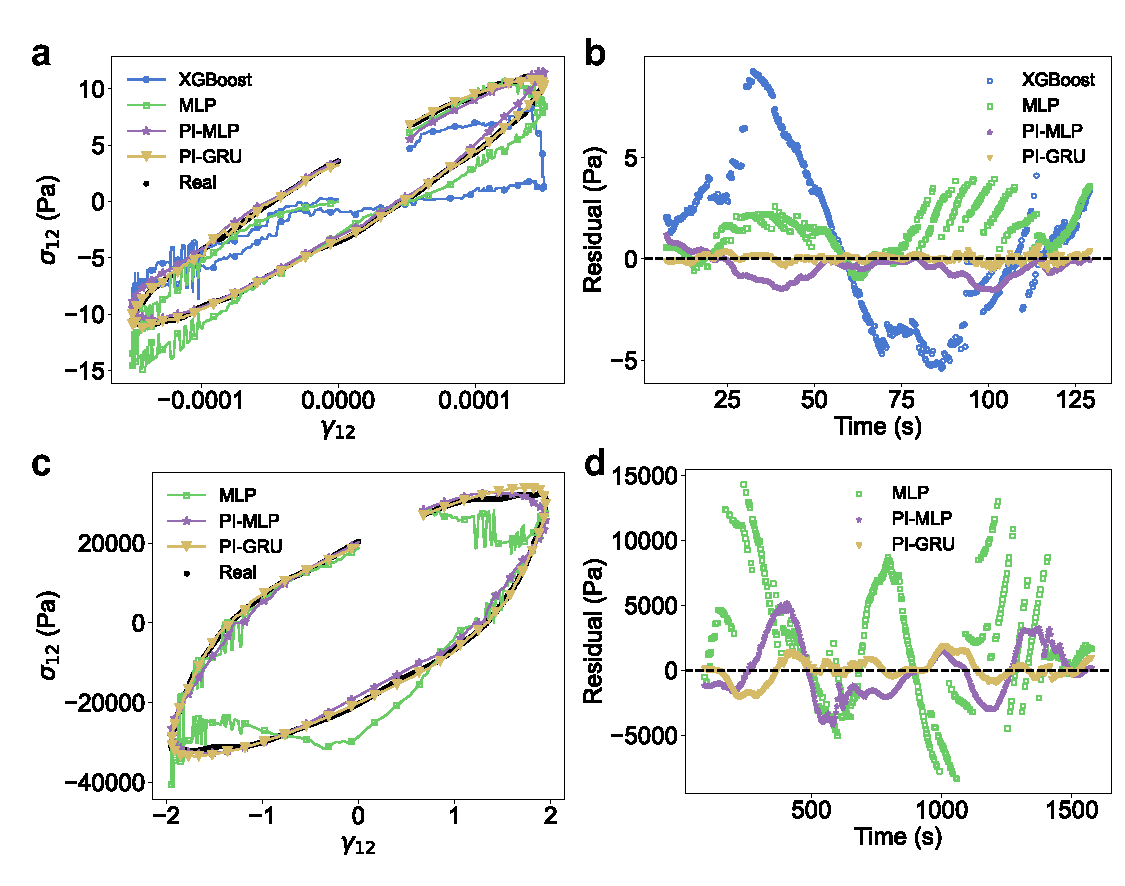
\includegraphics[width=0.9\textwidth]{Fig/real-data-differstrain.pdf}
  \FigureBicaption{\label{real-data-differstrain}ABE弹性体数据测试集上XGBoost、MLP、PI-MLP和PI-GRU模型的预测结果与真实数据对比,(a-b)为SAO测试集,训练数据与测试数据均为SAOS数据,而(c-d)为LAOS测试集,训练数据为SAOS数据和LAOS数据,测试数据为LAOS数据:(a)SAOS测试集剪切应力$\sigma_{12}$真实值与模型预测值的Lissajous曲线;(b)SAOS测试集剪切应力$\sigma_{12}$真实值与模型预测值的残差图;(c)LAOS测试集剪切应力$\sigma_{12}$真实值与模型预测值的Lissajous曲线;(d)LAOS测试集剪切应力$\sigma_{12}$真实值与模型预测值的残差图}{Comparison schematic of the prediction results of the XGBoost, MLP, PI-MLP, and PI-GRU models on the ABE elastomer data test set: (a-b) SAOS test set, both training and test data are SAOS data, and (c-d) LAOS test set, training data are SAOS data and LAOS data, test data are LAOS data: (a) Lissajous curve of the true value and predicted value of the shear stress $\sigma_{12}$ for the SAOS test set; (b) residual plot of the true value and predicted value of the shear stress $\sigma_{12}$ for the SAOS test set; (c) Lissajous curve of the true value and predicted value of the shear stress $\sigma_{12}$ for the LAOS test set; (d) residual plot of the true value and predicted value of the shear stress $\sigma_{12}$ for the LAOS test set}
  \label{real-data-differstrain}
\end{figure}
本研究选取的实验材料为一类具有黏弹性的ABE弹性体材料,具体材料情况在999节中详细介绍。
\subsubsection{SAOS数据预测}

\begin{figure}
  \centering
  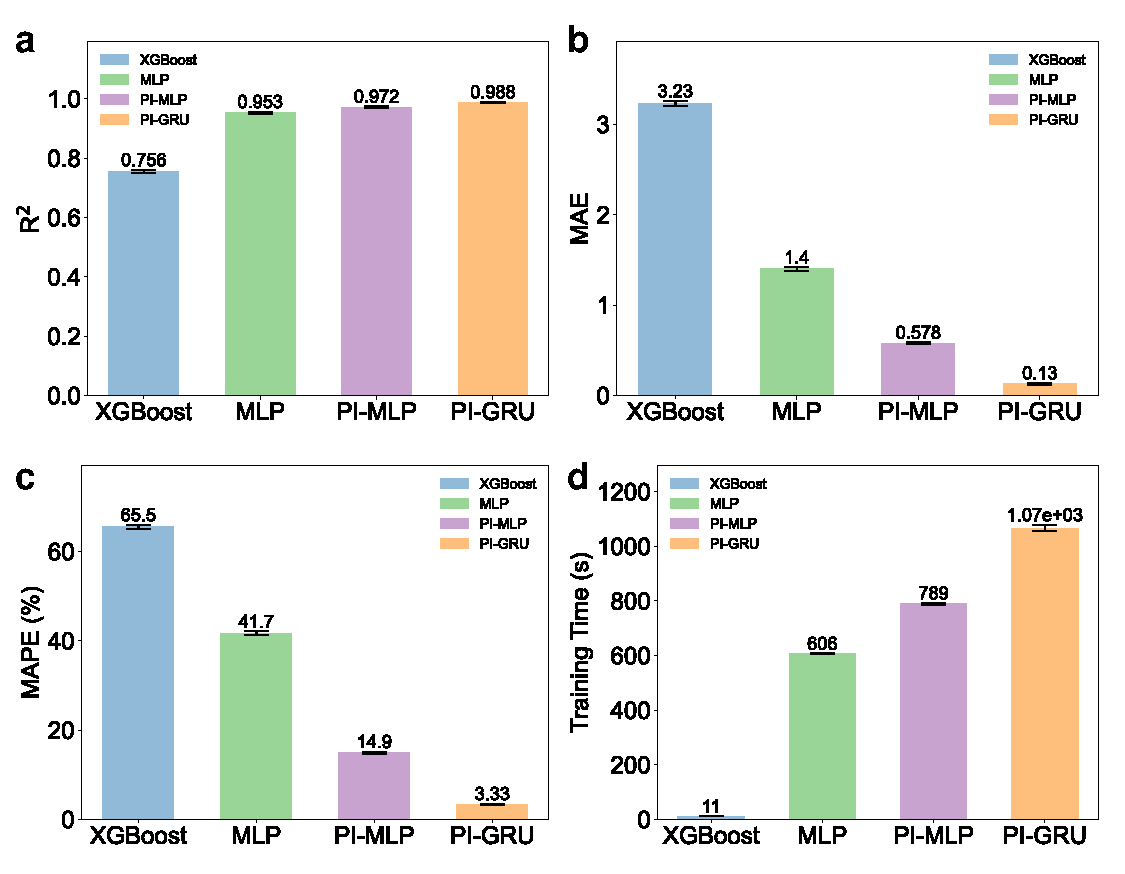
\includegraphics[width=0.9\textwidth]{Fig/real-data-differstrain-saos-metrics.pdf}
  \FigureBicaption{\label{real-data-differstrain-saos-metrics}ABE弹性体数据SAOS测试集上XGBoost、MLP、PI-MLP和PI-GRU模型的预测指标对比:(a)R$^2$值;(b)MAE值;(c)MAPE值;(d)训练时间}{Comparison schematic of the prediction metrics of the XGBoost, MLP, PI-MLP, and PI-GRU models on the ABE elastomer data SAOS test set: (a) R$^2$ value; (b) MAE value; (c) MAPE value; (d) training time}
\end{figure}
\begin{figure}
  \centering
  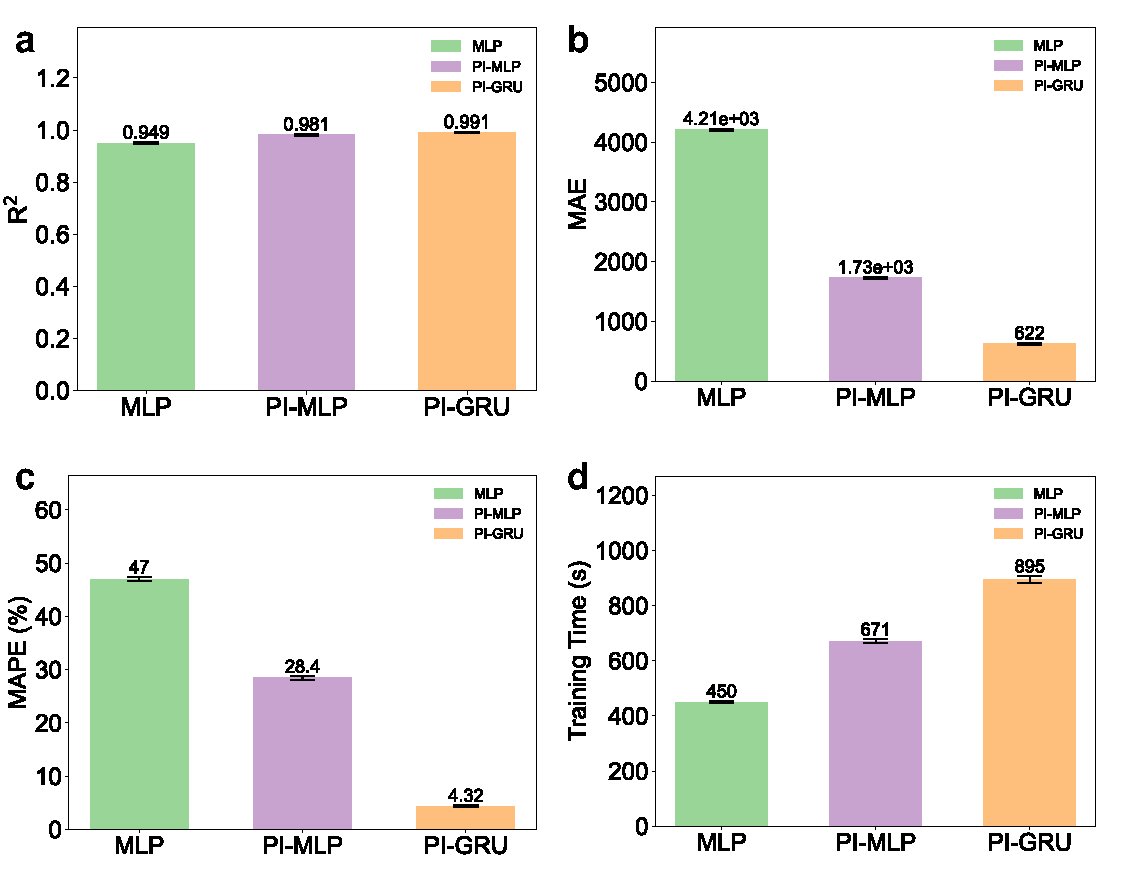
\includegraphics[width=0.9\textwidth]{Fig/real-data-differstrain-laos-metrics.pdf}
  \FigureBicaption{\label{real-data-differstrain-laos-metrics}ABE弹性体数据LAOS测试集上XGBoost、MLP、PI-MLP和PI-GRU模型的预测指标对比:(a)R$^2$值;(b)MAE值;(c)MAPE值;(d)训练时间}{Comparison schematic of the prediction metrics of the XGBoost, MLP, PI-MLP, and PI-GRU models on the ABE elastomer data LAOS test set: (a) R$^2$ value; (b) MAE value; (c) MAPE value; (d) training time}
\end{figure}
图\ref{real-data-differstrain}(a,b)和图\ref{real-data-differstrain-saos-metrics}展示了PI-GRU模型在真实数据集的SAOS数据上的预测结果,这里对比了XGBoost模型\cite{Goodfellow-et-al-2016},MLP模型,PI-MLP模型(增加物理约束,但使用MLP结构)和PI-GRU模型。
这里使用的物理约束为UCM模型,其表达式如公式\ref{eq:ucm}所示。

从真实-预测值曲线(图\ref{real-data-differstrain}a)和残差图(图\ref{real-data-differstrain}b)可以定性看出不同模型之间的预测效果是:PI-GRU>PI-MLP>MLP>XGBoost。从定量指标来看,纯数据驱动的XGBoost模型和MLP模型在预测真实数据时表现较差,MAPE指标均高于40\%,在物理约束的加持下,PI-MLP模型和PI-GRU模型在预测真实数据时表现较好,MAPE指标均低于20\%,其中PI-GRU模型在预测真实数据时表现最佳为3.33\%。而训练时间上,PI-GRU模型由于其循环神经网络结构特性,训练时间最高为1070 s。
本节的研究表明,PI-GRU模型在真实的SAOS数据上可以取得较好的预测效果,通过学习不同振幅的SAOS数据,模型可以学习到材料线性黏弹性特征,并泛化到未知应变协议的数据,这意味着只需有限的的流变学实验,便可以得到一个较为准确的某种材料的线性黏弹本构关系,从而为材料的设计和优化提供理论指导。
\subsubsection{LAOS数据预测}

在进一步的研究中,图\ref{real-data-differstrain}(c,d)和图\ref{real-data-differstrain-laos-metrics}展示了PI-GRU模型在真实数据集的LAOS数据上的预测结果,由于LAOS数据的测量难度和时间都高于SAOS且需要的样品量更多,这里的训练数据同时包含SAOS和LAOS数据,这里对比了MLP模型,PI-MLP模型和PI-GRU模型,其中PI-GRU模型预测的曲线与真实曲线最为吻合,图\ref{real-data-differstrain-laos-metrics}的预测相关指标显示PI-GRU在这项任务上的R$^2$为0.991,MAE值为622,MAPE值为4.32\%,均领先其他算法模型。

PI-GRU模型的优越性能源于其门控机制与黏弹性材料应力响应机制高度契合,可选择性保留或遗忘历史信息,而物理约束的引入使其遵循流变学原理,避免纯数据驱动方法的物理不一致性。通过SAOS与LAOS数据协同训练,模型可学习材料从线性到非线性区域的连续转变特性,构建完整响应图景,实现不同应变幅度和频率下的精准预测。这种基于"多尺度"学习的方法,在SAOS数据易获取、LAOS数据难获取的实际条件下,能高效建立黏弹性材料非线性本构关系,显著降低高分子加工领域的实验成本与时间,为材料开发和工艺优化提供高效数据支持。

\subsubsection{不同本构约束}
\begin{figure}
  \centering
  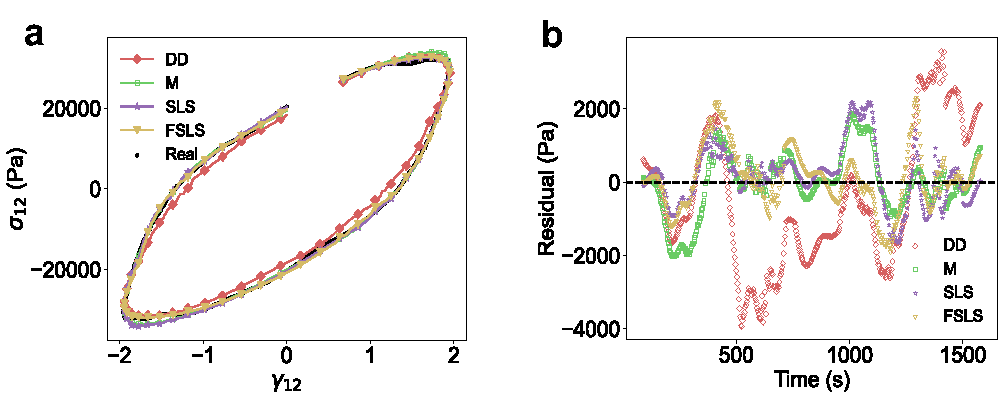
\includegraphics[width=0.9\textwidth]{Fig/real-data-differcons.pdf}
  \FigureBicaption{\label{real-data-differcons}ABE弹性体数据LAOS测试集使用不同本构方程作为物理约束的PI-GRU模型的预测效果对比,这里DD指的是没有物理约束的纯数据驱动模型,M代表的是Maxwell模型,SLS为标准线性固体模型,方程如\ref{eq:sls}所示,FSLS为分数阶线性固体模型,方程如\ref{eq:fsls}所示:(a)剪切应力$\sigma_{12}$真实值与模型预测值的Lissajous曲线;(b)剪切应力$\sigma_{12}$真实值与模型预测值的残差图}{Comparison schematic of the prediction results of the PI-GRU model with different constitutive equations as physical constraints on the ABE elastomer data LAOS test set. Here DD refers to a pure data-driven model without physical constraints, M represents the Maxwell model, SLS is the standard linear solid model as shown in equation \ref{eq:sls}, and FSLS is the fractional-order linear solid model as shown in equation \ref{eq:fsls}: (a) Lissajous curve of the true value and predicted value of the shear stress $\sigma_{12}$; (b) residual plot of the true value and predicted value of the shear stress $\sigma_{12}$}
\end{figure}
本研究使用的PI-GRU模型一个很重要的组件就是物理方程的约束,而PI-GRU作为物理信息机器学习(PIML)的一种,存在一个研究者都颇为关心的问题,即如何在一个具体的科学问题中从浩繁的物理方程中选择一个最适配的物理方程。为了了解PI-GRU模型对于本构方程的依赖性,本研究探究了不同本构方程作为物理约束下的建模预测效果。图\ref{real-data-differcons}和图\ref{real-data-differcons-metrics}展示了不同本构方程作为物理约束的PI-GRU的预测效果,其中纯数据驱动(DD)组的效果最差,这里本质上使用的GRU模型,与上文的结果不同,在真实的数据集上,单纯的GRU模型预测非线性区间的LAOS数据表现不佳,MAPE值高达36.4\%,这里考虑是真实场景下材料流变性质的复杂性超过有限参数的数值模拟数据。而引入物理约束后,模型的预测效果则得到较大提升,本节的工作中,M代表的是Maxwell模型,SLS为标准线性固体模型,方程如所示,FSLS为分数阶线性固体模型,方程如所示。
\begin{align}
  \sigma(t) + \lambda_{1} \frac{d \sigma(t)}{d t}            & = G \left( \gamma(t) + \lambda_2 \frac{d \gamma(t)}{d t} \right) (SLS) \label{eq:sls}             \\
  \sigma(t) + \lambda_1 \frac{d^\alpha \sigma(t)}{dt^\alpha} & = G \left( \gamma(t) + \lambda_2 \frac{d^\beta \gamma(t)}{dt^\beta} \right)(FSLS) \label{eq:fsls}
\end{align}

研究中使用的ABE弹性体是一类黏弹性固体材料,Maxwell模型在实践中多用于高分子流体的线性区间拟合,SLS模型则多用于黏弹性固体的线性区间拟合,FSLS模型通过分数阶导数的记忆性和幂律特性,突破了整数阶模型的指数衰减限制,兼容材料的长期记忆、宽弛豫时间分布和幂律响应等非线性特征\cite{ricarteTutorialReviewLinear2024,ewoldtDesigningComplexFluids2022}。这几个本构模型中理论上FSLS模型最能描述ABE弹性体的本构关系,而应用到PI-GRU的模型中,结果表明三种不同适配场景的本构方程作为物理约束情况下,最终的泛化预测效果非常接近,且没有呈现预期的梯度变化趋势。具体而言,在R$^2$指标上Maxwell模型约束的模型表现最优,在MAE指标上SLS模型略胜一筹,而在MAPE指标上Maxwell模型又占优势,但这些差异在统计学意义上并不显著。这一现象表明,PI-GRU模型在ABE弹性体流变数据建模过程中表现出一定程度的本构方程无关性,即使是理论上更适合流体而非固体的Maxwell方程作为物理约束,模型也能取得令人满意的预测效果。

PI-GRU的本构无关性可能源于物理信息与GRU网络结构之间的协同增强作用。图\ref{real-data-differstrain}的结果清晰地表明PI-GRU相比PI-MLP具有显著的预测优势,而图\ref{real-data-differcons}的结果则证实PI-GRU相比纯数据驱动的GRU模型有着本质的提升,这两组对比共同证明了物理约束和门控循环单元结构在提升预测性能方面均发挥着关键作用。物理约束为模型提供了一个基础的理论框架,使得模型不必严格符合特定材料的全部特性,只需满足黏弹性材料的基本数学假设;而GRU结构则通过其记忆机制有效捕捉了材料响应中的时间依赖性和非线性特征。这种设计理念与Mahmoudabadbozchelou和Jamali提出的MFNN或PINN模型有相似之处\cite{mahmoudabadbozchelouDatadrivenPhysicsinformedConstitutive2021},但PI-GRU模型通过其特殊的神经网络架构,有效地捕捉了时间域流变数据中的历史依赖性特征,在模型设计上更为贴近真实的黏弹性材料。

\begin{figure}
  \centering
  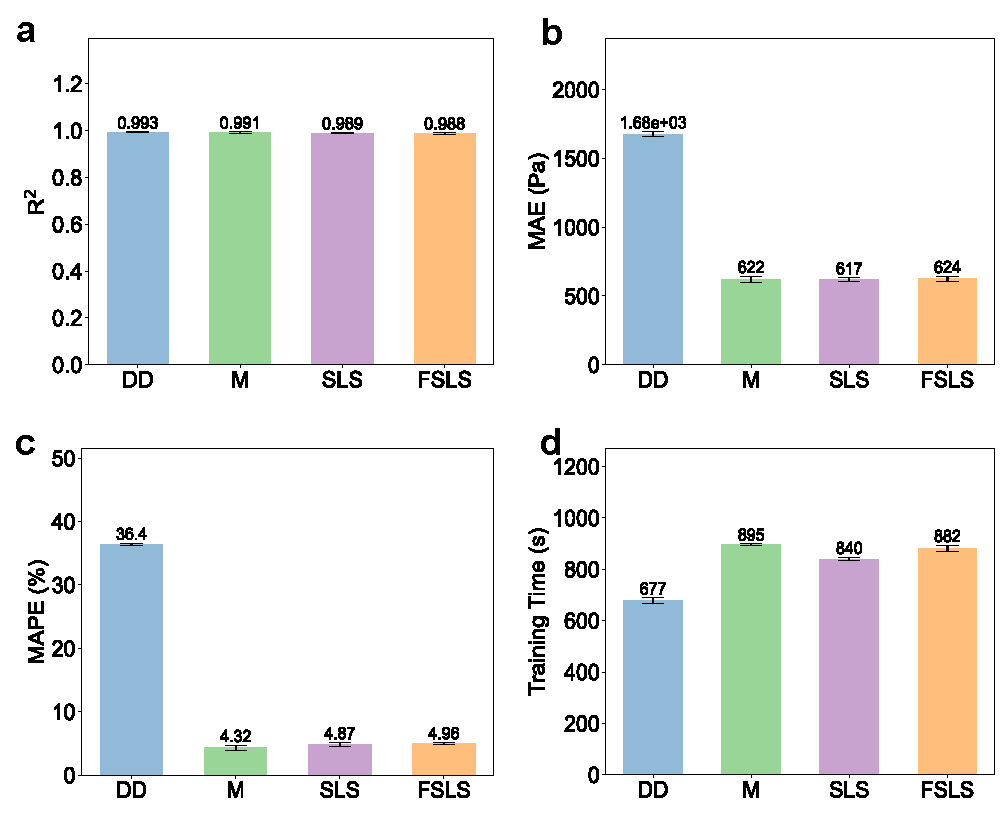
\includegraphics[width=0.9\textwidth]{Fig/real-data-differcons-metrics.pdf}
  \FigureBicaption{\label{real-data-differcons-metrics}ABE弹性体数据LAOS测试集使用不同本构方程作为物理约束的PI-GRU模型的预测指标对比:(a)R$^2$值;(b)MAE值;(c)MAPE值;(d)训练时间}{Comparison schematic of the prediction metrics of the PI-GRU model with different constitutive equations as physical constraints on the ABE elastomer data LAOS test set: (a) R$^2$ value; (b) MAE value; (c) MAPE value; (d) training time}
\end{figure}
Lennon等人提出的RUDE框架采用了Oldroyd形式的微分方程作为基础框架,Oldroyd形式的微分方程事实上已经包含时间依赖性,仅通过神经网络训练框架无法拟合的非线性部分,因此RUDE不需要事先确定精确的本构方程\cite{lennonScientificMachineLearning2023a}。相比之下,我们的PI-GRU模型将物理约束作为一个大致约束,依靠GRU的门控单元结构来学习材料的时间依赖性,本质上是将RUDE的设计以非解析方程的形式融入到模型中。

这一发现对于实际应用具有重要意义,它表明在使用PI-GRU模型进行黏弹性材料建模时,研究者可以选择相对简单的物理约束方程,而不必过分关注物理方程与材料特性的精确匹配度,这大大简化了模型的设计和应用过程。同时,这也为未来开发更通用的黏弹性材料建模框架提供了新的思路,即通过合理的神经网络结构设计,可以在一定程度上弥补物理模型的不足,实现更广泛的适用性。


% 本章小结 
\section{本章小结}

本章首先运用了GRU算法对数值模拟的 Herschel-Bulkley 模型、Maxwell 模型以及Doi-Edwards 模型所产生的模拟数据展开深度学习建模工作。

研究结果揭示出,GRU 作为一种循环神经网络,依托其独特的门控单元机制,能够精准地捕捉黏弹性材料流变学模拟数据所蕴含的时间依赖性以及复杂非线性特征。特别的,在处理 Herschel-Bulkley 模型这类非时间序列数据时,GRU 模型的预测效果相较于DNN模型依旧略胜一筹。究其原因,在于 GRU 的门控单元机制引入了更多的参数,从而赋予了其更佳的泛化性能。对于经典的简单 Maxwell模型,由于属于典型的时间序列数据,GRU对其进行建模预测的效果全面超越DNN,各项评估指标均展现出显著优势。当面对更为复杂Doi-Edwards 模型时,GRU的建模预测效果依旧优于 DNN。进一步分析发现,在相同的建模任务中,GRU 在剪切应力$\sigma_{12}$的预测效果上强于第一法向应力差$N_1$。

在本章模拟数据预测部分设计的实验中,我们探讨了两类预测任务:首先,利用交变应变变化的训练数据,预测相应的测试数据;其次,使用交变应变变化实验的训练数据,预测稳态剪切的测试数据。在针对不同本构模型的这两类实验中,GRU模型的表现均优于DNN。这一现象充分表明,GRU具备更强的泛化能力,能够有效地预测更为一般化的本构关系,而不仅仅是进行简单的函数逼近。GRU通过引入门控机制,能够有效捕捉序列数据中的长期依赖关系,从而在处理复杂的本构模型时展现出更优的性能。相比之下,DNN虽然在非时序本构模型中表现出色,但在处理具有复杂时序特征的本构模型时,其性能会受到限制。因此,选择GRU模型进行本构关系的预测,能够更好地适应数据的复杂性和多样性,提升预测的准确性和可靠性,但是本章的实验结果同样表明,GRU模型由于其架构特征,比普通DNN的训练时间高很多,且训练时消耗更多的计算机资源(计算机内存、GPU显存等)。

综上所述,本章的研究工作充分验证了GRU在流变学数据建模中的优异效果。该模型不仅能够准确捕捉黏弹性材料的时间依赖性,从而高效刻画非线性、时变的物理过程,展现出良好的关联适配性,而且在理论上突破了传统数据拟合方法的局限,在模拟数据和真实实验数据中均表现出卓越的泛化能力和预测稳定性。总的来说,本章的研究为深度学习在流变学本构建模领域的应用开辟了全新的思路,即可以从模型升级的角度去优化本构建模的过程。





